% =============================================================================
% WEAPON-TARGET ASSIGNMENT PROBLEM - Checkpoint 2 Presentation
% Algorithm Engineering Sessional - CSE 462, Group 5
% =============================================================================

\documentclass[aspectratio=43,8pt]{beamer}

% =============================================================================
% THEME AND COLORS
% =============================================================================
\usetheme{default}
\usecolortheme{default}

% Professional minimal color scheme - muted grayscale
\definecolor{primaryblue}{RGB}{40, 40, 40}
\definecolor{secondaryblue}{RGB}{80, 80, 80}
\definecolor{accentred}{RGB}{100, 100, 100}
\definecolor{accentgreen}{RGB}{60, 60, 60}
\definecolor{lightgray}{RGB}{200, 250, 200}

\setbeamercolor{structure}{fg=primaryblue}
\setbeamercolor{frametitle}{bg=white, fg=primaryblue}
\setbeamercolor{title}{fg=primaryblue}
\setbeamercolor{block title}{bg=lightgray, fg=primaryblue}
\setbeamercolor{block body}{bg=white}
\setbeamercolor{block title alerted}{bg=lightgray, fg=primaryblue}
\setbeamercolor{block title example}{bg=lightgray, fg=primaryblue}

% Simplify itemize bullets
\setbeamertemplate{itemize items}[circle]
\setbeamertemplate{enumerate items}[default]

% Remove shadows and rounded corners for cleaner look
\setbeamertemplate{blocks}[default]
\setbeamertemplate{title page}[default][colsep=-4bp,rounded=false]

% Minimal navigation
\setbeamertemplate{navigation symbols}{}

% Clean frame title with reduced spacing
\setbeamertemplate{frametitle}{
  \vspace{0.2cm}
  \insertframetitle
  \vspace{0.05cm}
  \hrule
  \vspace{0.2cm}
}

% Maximize content area - reduce margins and spacing
\setbeamersize{text margin left=0.5cm,text margin right=0.5cm}
\setlength{\parskip}{3pt}

% =============================================================================
% PACKAGES
% =============================================================================
\usepackage[utf8]{inputenc}
\usepackage[T1]{fontenc}
\usepackage{lmodern}
\usepackage{amsmath}
\usepackage{amssymb}
\usepackage{graphicx}
\usepackage{booktabs}
\usepackage{array}
\usepackage{tikz}
\usetikzlibrary{positioning, arrows.meta, shapes, calc}
\usepackage{algorithm}
\usepackage{algpseudocode}
\usepackage{xcolor}
\usepackage{hyperref}
\usepackage{multirow}

% =============================================================================
% FOOTER CONFIGURATION
% =============================================================================
\setbeamertemplate{navigation symbols}{}
\setbeamertemplate{footline}{
  \hfill\usebeamerfont{page number in head/foot}\insertframenumber{} / \inserttotalframenumber\hspace*{1em}\vskip2pt
}

% =============================================================================
% TITLE INFORMATION
% =============================================================================
\title[WTA Problem]{\textbf{Weapon-Target Assignment Problem}}
\subtitle{Algorithm Engineering Sessional -- Checkpoint 2 Presentation}
\author[Team WTA]{Team Members}
\institute[CSE 462]{CSE 462: Algorithm Engineering Sessional}
\date{March 2026}

% =============================================================================
% DOCUMENT BEGINS
% =============================================================================
\begin{document}

% =============================================================================
% TITLE SLIDE
% =============================================================================
\begin{frame}[plain]
\begin{center}
\vspace{0.3cm}
% BUET Logo

\includegraphics[width=0.15\textwidth]{images/buet_logo.png}

\vspace{0.3cm}
{\Large\textbf{\textcolor{primaryblue}{Weapon-Target Assignment Problem}}}

\vspace{0.3cm}
{\normalsize CSE 462: Algorithm Engineering Sessional}

{\normalsize Checkpoint 2 Presentation}

\vspace{0.5cm}
\begin{tabular}{ll}
\textbf{Team Members} & \\
Hozifa Rahman Hamim & (ID: 1705083) \\
Md. Azizul Haque Nadim & (ID: 1905059) \\
Sadia Tabassum & (ID: 1905091) \\
Ahmmad Nur Swapnil & (ID: 2005009) \\
Most. Sonia Khatun & (ID: 2005025) \\
Shahriar Ahmed Seam & (ID: 2005093) \\
\end{tabular}

\vspace{0.5cm}
{\small Department of Computer Science and Engineering (CSE)}

{\small Bangladesh University of Engineering and Technology (BUET)}

\vspace{0.3cm}
{\footnotesize\textit{March 2026}}
\end{center}
\end{frame}

% =============================================================================
% REAL-WORLD WTA EXAMPLES SLIDE
% =============================================================================
\begin{frame}{Real-World Motivation: WTA in Action}
\begin{columns}[t]
\column{0.48\textwidth}
\begin{center}
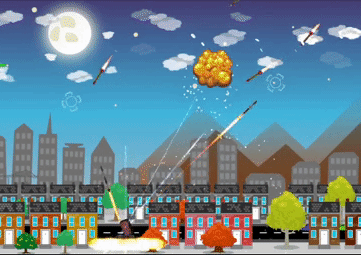
\includegraphics[width=0.95\textwidth]{images/iron_dome_image.png}

{\footnotesize\textbf{Air Defense (Iron Dome)}}
\end{center}

\vspace{0.1cm}
{\scriptsize\textbf{WTA Mapping:}}
\begin{itemize}\setlength{\itemsep}{0pt}
    \item[\textcolor{blue}{$\bullet$}] Interceptor Missiles = \textbf{Weapons}
    \item[\textcolor{red}{$\bullet$}] Incoming Rockets = \textbf{Targets}
    \item[\textcolor{green!60!black}{$\rightarrow$}] Assignment = \textbf{WTA Solution}
\end{itemize}

\column{0.52\textwidth}
\begin{center}
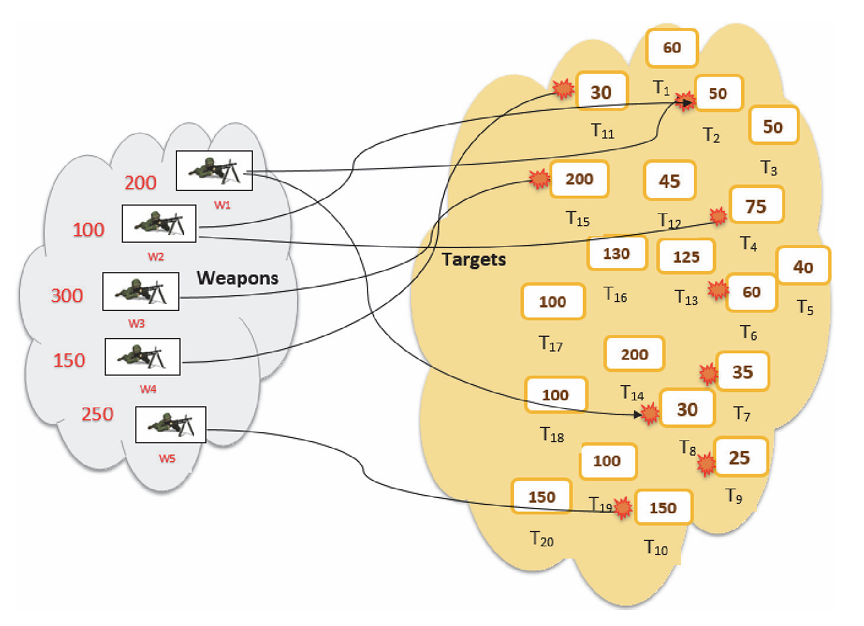
\includegraphics[width=0.95\textwidth]{images/ground_attack_image.png}

{\footnotesize\textbf{Ground Attack Scenario}}
\end{center}

\vspace{0.1cm}
{\scriptsize\textbf{WTA Mapping:}}
\begin{itemize}\setlength{\itemsep}{0pt}
    \item[\textcolor{blue}{$\bullet$}] W1--W5 (with costs) = \textbf{Weapons}
    \item[\textcolor{red}{$\bullet$}] T1--T20 (with values) = \textbf{Targets}
    \item[\textcolor{green!60!black}{$\rightarrow$}] Arrows = \textbf{Assignments}
\end{itemize}
\end{columns}
\end{frame}

% =============================================================================
% OUTLINE SLIDE
% =============================================================================
\begin{frame}{Presentation Outline}
\begin{columns}[t]
\column{0.48\textwidth}
\begin{block}{Part 1: Theory \& Background}
\begin{enumerate}
    \item \textbf{Problem Definition}
    \begin{itemize}
        \item Formal definition \& formulation
        \item Classifications
    \end{itemize}
    \item \textbf{NP-Hardness Proofs}
    \begin{itemize}
        \item Reduction from SUBSET PRODUCT
        \item Reduction to Multiple Knapsack
    \end{itemize}
    \item \textbf{Algorithm Survey}
    \begin{itemize}
        \item Exact, approximation, heuristic, metaheuristic
    \end{itemize}
\end{enumerate}
\end{block}

\column{0.48\textwidth}
\begin{block}{Part 2: Implementation \& Results}
\begin{enumerate}
\setcounter{enumi}{3}
    \item \textbf{Selected Algorithms}
    \begin{itemize}
        \item Maximum Marginal Return (MMR)
        \item Genetic Algorithm (GA)
    \end{itemize}
    \item \textbf{Our Modifications}
    \begin{itemize}
        \item MMR-IR: local search enhancement
        \item Hybrid GA: 3 novel modifications
    \end{itemize}
    \item \textbf{Experiments \& Results}
    \begin{itemize}
        \item 180 instances, 9 plots, statistics
    \end{itemize}
\end{enumerate}
\end{block}
\end{columns}
\end{frame}

% =============================================================================
% SECTION 1: PROBLEM DEFINITION
% =============================================================================
\section{Problem Definition}

\begin{frame}{Section 1: Problem Definition}
\begin{center}
{\Large\textcolor{primaryblue}{\textbf{What is the Weapon-Target Assignment Problem?}}}

\vspace{0.5cm}
{\normalsize A fundamental combinatorial optimization problem in operations research}
\end{center}
\end{frame}

\begin{frame}{Problem Definition}
\begin{block}{Weapon-Target Assignment (WTA) Problem}
The WTA problem involves the \textbf{strategic allocation of a set of weapons to a set of targets} to achieve a specific defensive or offensive objective.
\end{block}

\vspace{0.3cm}
\begin{alertblock}{Core Challenge: Stochastic Nature of Combat}
Every engagement is modeled as a \textbf{probabilistic event} where a weapon has a specific likelihood of destroying its assigned target.
\end{alertblock}

\vspace{0.3cm}
\begin{exampleblock}{Computational Complexity}
\begin{itemize}
    \item The problem is mathematically proven to be \textbf{NP-complete}
    \item As the number of weapons and targets grows, complexity increases \textbf{exponentially}
    \item Finding an absolute optimal solution becomes extremely difficult for large instances
\end{itemize}
\end{exampleblock}
\end{frame}

\begin{frame}{Classification: Asset-based vs. Target-based}
\begin{block}{Two Perspectives of WTA}
The WTA problem can be viewed from two distinct perspectives depending on whether the objective prioritizes \textbf{destruction of enemy forces} or \textbf{protection of friendly resources}.
\end{block}

\vspace{0.3cm}
\begin{columns}[t]
\column{0.48\textwidth}
\begin{alertblock}{Target-based Perspective}
Values assigned to each \textbf{enemy target} based on threat they pose.
\begin{itemize}
    \item \textbf{Goal:} Maximize total damage inflicted on incoming targets
    \item \textbf{Math:} \textbf{Minimize} expected survival value of targets
    \item (Equivalent to maximizing damage)
\end{itemize}
\end{alertblock}

\column{0.48\textwidth}
\begin{exampleblock}{Asset-based Perspective}
Values assigned to \textbf{defended assets} (cities, bases) rather than targets.
\begin{itemize}
    \item \textbf{Goal:} Maximize combined survival value of friendly assets
    \item \textbf{Requirement:} Map which targets attack which assets
    \item \textbf{Math:} \textbf{Maximize} expected value of surviving assets
\end{itemize}
\end{exampleblock}
\end{columns}
\end{frame}

\begin{frame}{Mathematical Representation: Parameters and Variables}
\begin{block}{Target-based Formulation -- Parameters}
\begin{itemize}
    \item $W = \{1, \dots, m\}$: The set of available \textbf{weapons}
    \item $T = \{1, \dots, n\}$: The set of \textbf{targets} to be engaged
    \item $V_j$: The \textbf{strategic military value} or importance of target $j$
    \item $p_{ij}$: The ``\textbf{probability of kill}'' -- chance that weapon $i$ will destroy target $j$
\end{itemize}
\end{block}

\vspace{0.3cm}
\begin{exampleblock}{Decision Variable}
$$x_{ij} \in \{0, 1\}$$
\textbf{Binary variable:} $x_{ij} = 1$ if weapon $i$ is assigned to target $j$, 0 otherwise.

Each weapon is assigned to exactly one target.
\end{exampleblock}
\end{frame}

\begin{frame}{Mathematical Representation: Objective Functions}
\begin{block}{Goal: Maximize damage (or equivalently, minimize survival)}
While the goal is to maximize damage, the standard convention is to minimize remaining survival value.
\end{block}

\vspace{0.2cm}
\begin{columns}[t]
\column{0.48\textwidth}
\begin{alertblock}{1. Maximizing Total Expected Damage}
\begin{equation*}
\text{Max } Z = \sum_{j=1}^{n} V_j \left[ 1 - \prod_{i=1}^{m} (1 - p_{ij})^{x_{ij}} \right]
\end{equation*}
\end{alertblock}

\column{0.48\textwidth}
\begin{exampleblock}{2. Minimizing Expected Survival Value}
\begin{equation*}
\text{Min } Z = \sum_{j=1}^{n} V_j \prod_{i=1}^{m} (1 - p_{ij})^{x_{ij}}
\end{equation*}
\end{exampleblock}
\end{columns}

\vspace{0.3cm}
\begin{block}{Key Insight}
$\prod_{i=1}^{m} (1 - p_{ij})^{x_{ij}}$ = \textbf{Probability that target $j$ survives ALL assigned weapons}

The product captures the \textbf{combined effect} of multiple weapons attacking the same target.
\end{block}
\end{frame}

\begin{frame}{Mathematical Representation: Constraints}
\begin{block}{Constraint 1: Each Weapon Assigned Once}
\begin{equation*}
\sum_{j=1}^{n} x_{ij} = 1, \quad \forall i \in W
\end{equation*}
\textbf{Meaning:} Every weapon must be assigned to exactly one target.
\end{block}

\vspace{0.3cm}
\begin{alertblock}{Constraint 2: Integrality}
\begin{equation*}
x_{ij} \in \{0, 1\}
\end{equation*}
\textbf{Meaning:} Binary assignment -- weapon $i$ is either assigned to target $j$ or not.
\end{alertblock}

\vspace{0.3cm}
\begin{exampleblock}{Complete Formulation Summary}
\textbf{Minimize} $\sum_{j} V_j \prod_{i} (1-p_{ij})^{x_{ij}}$ \quad
\textbf{s.t.} $\sum_{j} x_{ij} = 1$, \quad $x_{ij} \in \{0,1\}$
\end{exampleblock}
\end{frame}

\begin{frame}{Linear vs. Non-Linear Assignment}
\begin{columns}[t]
\column{0.48\textwidth}
\begin{block}{Linear Assignment Problem (LAP)}
\begin{itemize}
    \item \textbf{Structure:} One weapon assigned to exactly one target (\textbf{One-to-One})
    \item \textbf{Linearity:} Objective function is linear
    \item Assignments are \textbf{independent}
    \item \textcolor{accentgreen}{\textbf{Polynomial time solvable}} (Hungarian algorithm)
\end{itemize}
\end{block}

\column{0.48\textwidth}
\begin{alertblock}{Non-Linear Assignment (Non-LAP)}
\begin{itemize}
    \item \textbf{Structure:} Multiple weapons can be assigned to single target (\textbf{Many-to-One})
    \item \textbf{Non-Linearity:} Due to ``\textbf{diminishing returns}''
    \item Additional weapons = \textbf{overkill} effect
    \item \textcolor{accentred}{\textbf{NP-complete!}}
\end{itemize}
\end{alertblock}
\end{columns}

\vspace{0.3cm}
\begin{center}
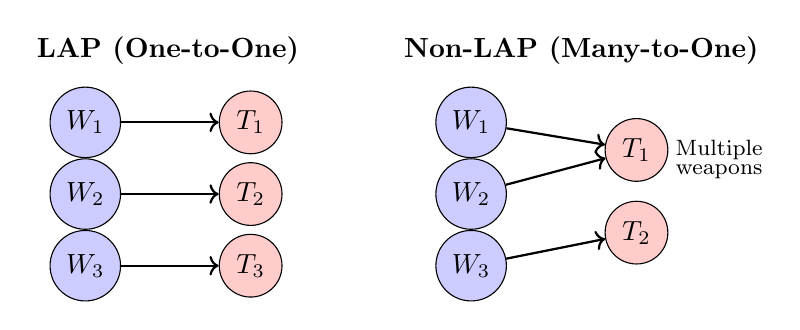
\begin{tikzpicture}[scale=0.7]
% LAP
\node at (-3.5, 1.8) {\textbf{LAP (One-to-One)}};
\node[circle, draw, fill=blue!20, minimum size=0.6cm] (w1) at (-5, 0.5) {$W_1$};
\node[circle, draw, fill=blue!20, minimum size=0.6cm] (w2) at (-5, -0.8) {$W_2$};
\node[circle, draw, fill=blue!20, minimum size=0.6cm] (w2b) at (-5, -2.1) {$W_3$};
\node[circle, draw, fill=red!20, minimum size=0.6cm] (t1) at (-2, 0.5) {$T_1$};
\node[circle, draw, fill=red!20, minimum size=0.6cm] (t2) at (-2, -0.8) {$T_2$};
\node[circle, draw, fill=red!20, minimum size=0.6cm] (t2b) at (-2, -2.1) {$T_3$};
\draw[->, thick] (w1) -- (t1);
\draw[->, thick] (w2) -- (t2);
\draw[->, thick] (w2b) -- (t2b);

% Non-LAP
\node at (4, 1.8) {\textbf{Non-LAP (Many-to-One)}};
\node[circle, draw, fill=blue!20, minimum size=0.6cm] (w3) at (2, 0.5) {$W_1$};
\node[circle, draw, fill=blue!20, minimum size=0.6cm] (w4) at (2, -0.8) {$W_2$};
\node[circle, draw, fill=blue!20, minimum size=0.6cm] (w5) at (2, -2.1) {$W_3$};
\node[circle, draw, fill=red!20, minimum size=0.6cm] (t3) at (5, 0) {$T_1$};
\node[circle, draw, fill=red!20, minimum size=0.6cm] (t4) at (5, -1.5) {$T_2$};
\draw[->, thick] (w3) -- (t3);
\draw[->, thick] (w4) -- (t3);
\draw[->, thick] (w5) -- (t4);
\node at (6.5, 0) {\footnotesize Multiple};
\node at (6.5, -0.4) {\footnotesize weapons};
\end{tikzpicture}
\end{center}
\end{frame}

% =============================================================================
% SECTION 2: NP-HARDNESS PROOFS
% =============================================================================
\section{NP-Hardness Proofs}

\begin{frame}{Section 2: NP-Hardness Proofs}
\begin{center}
{\Large\textcolor{primaryblue}{\textbf{Polynomial-Time Reductions}}}

\vspace{0.5cm}
{\normalsize Proving WTA is NP-complete through formal reductions}
\end{center}
\end{frame}

\begin{frame}{WTA Decision Problem}
\begin{block}{Decision Version of WTA}
\textbf{Given:}
\begin{itemize}
    \item Survival probability $q_{i,j} = 1 - p_{i,j}$
    \item Threshold value $k$
\end{itemize}

\textbf{Question:} Does there exist an assignment $x_{i,j} \in \{0,1\}$ such that:
\begin{equation*}
D = \sum_{j=1}^n V_j \prod_{i=1}^m q_{i,j}^{x_{i,j}} \leq k
\end{equation*}
\end{block}

\begin{alertblock}{Subject to Constraints}
$$\sum_{j=1}^n x_{i,j} \leq W_i \quad \text{for } i = 1, \ldots, m$$
$$x_{i,j} \in \{0, 1\}$$
where $x_{i,j} = 1$ if weapon $i$ assigned to target $j$, and $x_{i,j} = 0$ otherwise.

$D$ represents \textbf{total expected damage} (weighted survival probability of all targets)
\end{alertblock}
\end{frame}

\begin{frame}{Two Polynomial-Time Reductions}
\begin{block}{Our Approach}
We demonstrate two polynomial-time reductions:
\end{block}

\vspace{0.3cm}
\begin{columns}[t]
\column{0.48\textwidth}
\begin{alertblock}{Reduction 1}
\textbf{SUBSET PRODUCT $\leq_p$ WTA}

\vspace{0.2cm}
$\Rightarrow$ Proves \textbf{WTA is NP-hard}

\vspace{0.2cm}
{\small (Reduce FROM a known NP-complete problem TO WTA)}
\end{alertblock}

\column{0.48\textwidth}
\begin{exampleblock}{Reduction 2}
\textbf{WTA $\leq_p$ Multiple Knapsack}

\vspace{0.2cm}
$\Rightarrow$ Shows WTA reduces to another known NP-hard problem

\vspace{0.2cm}
{\small (Shows connection between problems)}
\end{exampleblock}
\end{columns}

\vspace{0.5cm}
\begin{center}
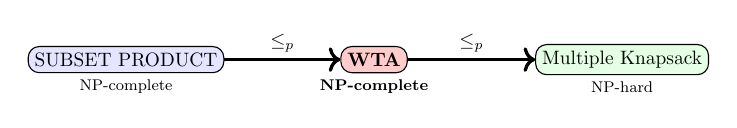
\begin{tikzpicture}[scale=0.7, transform shape]
\node[draw, rounded corners, fill=blue!10] (sp) at (0,0) {SUBSET PRODUCT};
\node[draw, rounded corners, fill=red!20] (wta) at (4.5,0) {\textbf{WTA}};
\node[draw, rounded corners, fill=green!10] (mk) at (9,0) {Multiple Knapsack};
\draw[->, very thick] (sp) -- node[above] {$\leq_p$} (wta);
\draw[->, very thick] (wta) -- node[above] {$\leq_p$} (mk);
\node[below] at (sp.south) {\footnotesize NP-complete};
\node[below] at (wta.south) {\footnotesize \textbf{NP-complete}};
\node[below] at (mk.south) {\footnotesize NP-hard};
\end{tikzpicture}
\end{center}
\end{frame}

\begin{frame}{Reduction 1: SUBSET PRODUCT $\leq_p$ WTA}
\begin{block}{SUBSET PRODUCT Problem (NP-complete)}
\textbf{Given:} Set $A = \{a_1, a_2, \ldots, a_m\}$ and target product $b$

\textbf{Find:} Subset $X \subseteq A$ where $\prod_{x \in X} a_x = b$
\end{block}

\vspace{0.2cm}
\begin{exampleblock}{WTA Instance Construction}
Let $P = \prod_{i=1}^m a_i$. Construct WTA with:
\begin{itemize}
    \item \textbf{Targets:} 2 targets with values $V_1 = V_2 = P$
    \item \textbf{Weapons:} $m + 2$ weapons: $W_1, W_2, \ldots, W_m, W_\alpha, W_\beta$
    \item \textbf{Survival probabilities:}
    \begin{columns}
    \column{0.45\textwidth}
    \begin{itemize}
        \item $q_{i,1} = q_{i,2} = \frac{1}{a_i}$ for $i = 1, \ldots, m$
    \end{itemize}
    \column{0.45\textwidth}
    \begin{itemize}
        \item $q_{\alpha,1} = q_{\alpha,2} = \frac{b}{2P}$
        \item $q_{\beta,1} = q_{\beta,2} = \frac{1}{2b}$
    \end{itemize}
    \end{columns}
    \item \textbf{Threshold:} $k = 1$ (we ask if $D \leq 1$)
\end{itemize}
\end{exampleblock}

\begin{alertblock}{Time Complexity}
Constructs WTA with 2 targets and $m+2$ weapons in $O(m)$ time -- \textbf{Polynomial!}
\end{alertblock}
\end{frame}

\begin{frame}{Reduction 1: Forward Direction}
\begin{block}{Forward ($\Rightarrow$): SUBSET PRODUCT has solution $\Rightarrow$ WTA has solution}
Suppose $X \subseteq \{1, \ldots, m\}$ with $\prod_{x \in X} a_x = b$. Let $Y = \{1, \ldots, m\} \setminus X$.

Then:
$$\prod_{i \in X} \frac{1}{a_i} = \frac{1}{b}, \quad \prod_{y \in Y} \frac{1}{a_y} = \frac{b}{P}$$

\textbf{Assignment:} $\{W_x : x \in X\} \cup \{W_\alpha\} \rightarrow T_1$ and $\{W_y : y \in Y\} \cup \{W_\beta\} \rightarrow T_2$

\textbf{Total damage:}
\begin{align*}
D &= V_1 \cdot \frac{b}{2P} \cdot \frac{1}{b} + V_2 \cdot \frac{1}{2b} \cdot \frac{b}{P} \\
&= P \cdot \frac{b}{2P} \cdot \frac{1}{b} + P \cdot \frac{1}{2b} \cdot \frac{b}{P} = \frac{1}{2} + \frac{1}{2} = 1 \leq k \quad \checkmark
\end{align*}
\end{block}
\end{frame}

\begin{frame}{Reduction 1: Backward Direction (Part 1)}
\begin{block}{Backward ($\Leftarrow$): WTA has solution $\Rightarrow$ SUBSET PRODUCT has solution}
Suppose WTA has solution with $D \leq 1$. Let $X', Y'$ be weapons assigned to $T_1, T_2$.
\end{block}

\begin{alertblock}{Claim: $W_\alpha$ and $W_\beta$ cannot both target the same target}
\textit{Proof:} If both assigned to $T_1$ (symmetric for $T_2$):
$$D \geq P \cdot \frac{1}{2b} \cdot \frac{b}{2P} \cdot \frac{1}{\prod_{x \in X' \setminus \{\alpha, \beta\}} a_x} + \frac{P}{\prod_{y \in Y'} a_y} \geq \frac{1}{4} + 1 > 1 \quad \Rightarrow\!\Leftarrow$$

So $W_\alpha \to T_1$ and $W_\beta \to T_2$. Let $X = X' \setminus \{\alpha\}$, $Y = Y' \setminus \{\beta\}$.
\end{alertblock}

\begin{block}{From the Assignment}
With $W_\alpha \to T_1$ and $W_\beta \to T_2$:
$$D = P \cdot \frac{b}{2P} \prod_{x \in X} \frac{1}{a_x} + P \cdot \frac{1}{2b} \prod_{y \in Y} \frac{1}{a_y} \leq 1$$
\end{block}

\end{frame}

\begin{frame}{Reduction 1: Backward Direction (Part 2)}

\begin{exampleblock}{Algebraic Derivation}
Let $z = \prod_{x \in X} a_x$. Then:
$$\frac{b}{2z} + \frac{z}{2b} \leq 1$$

Multiply by $2bz > 0$:
$$b^2 + z^2 \leq 2bz \quad \Rightarrow \quad (b - z)^2 \leq 0$$

Since $(b-z)^2 \geq 0$, we must have $(b-z)^2 = 0$, so:
$$b = z = \prod_{x \in X} a_x$$
\end{exampleblock}

\begin{alertblock}{Conclusion}
$X$ is a valid solution to SUBSET PRODUCT! $\checkmark$

\textbf{Time Complexity:} $O(m)$ -- Polynomial reduction complete.
\end{alertblock}
\end{frame}

\begin{frame}{Reduction 2: WTA $\leq_p$ Multiple Knapsack}
\begin{block}{Multiple Knapsack Construction}
Given WTA with $m$ targets, $n$ weapons, probabilities $\{p_{i,j}\}$:
\begin{itemize}
    \item \textbf{Knapsacks:} $m$ knapsacks (one per target) with Capacity $C_j = \infty$
    \item \textbf{Items:} $w_i$ items for weapon type $i$ (one per copy)
    \item \textbf{Profit:} $v_{ij} = -\log(1 - p_{i,j}) = -\log(q_{i,j})$
    \item \textbf{Question:} Does assignment with value $\geq V$ exist?
\end{itemize}
\end{block}

\begin{exampleblock}{Objective Transformation (Key Insight)}
For single target $j$, minimizing $\prod q_{i,j}^{x_{i,j}}$ equals minimizing:
$$\log\left(\prod_{i=1}^n q_{i,j}^{x_{i,j}}\right) = \sum_{i=1}^n x_{i,j} \log(q_{i,j})$$

Equivalent to \textbf{maximizing}:
$$-\sum_{i=1}^n x_{i,j} \log(q_{i,j}) = \sum_{i=1}^n x_{i,j} \cdot v_{ij}$$

This is \textbf{exactly the Multiple Knapsack objective!}
\end{exampleblock}
\end{frame}

\begin{frame}{Reduction 2: Constraint Mapping \& Conclusion}

\begin{block}{Constraint Mapping}
\begin{itemize}
    \item \textbf{WTA constraint:} $\sum_{j=1}^m x_{i,j} \leq W_i$ (weapon type $i$ used at most $W_i$ times)
    \item \textbf{Maps to:} $\sum_{j=1}^m y_{ij} \leq 1$ (each item in at most one knapsack) when $W_i = 1$
    \item For general $W_i$: Create $W_i$ copies of item $i$
\end{itemize}
\end{block}

\begin{exampleblock}{Equivalence}
Assignment $x_{i,j}$ optimal for WTA $\Leftrightarrow$ $y_{ij} = x_{i,j}$ optimal for Multiple Knapsack

\textbf{Logarithmic transformation preserves ordering of solutions!}

\textbf{Time:} $O(nm)$ to compute all $v_{ij} = -\log(1 - p_{i,j})$
\end{exampleblock}

\begin{alertblock}{Final Conclusion}
\begin{center}
\textbf{WTA is in NP} (solution verifiable in polynomial time) + \textbf{WTA is NP-hard}

$\Rightarrow$ \textbf{The Weapon-Target Assignment Problem is NP-complete!}
\end{center}
\end{alertblock}
\end{frame}

% =============================================================================
% SECTION 3: ALGORITHM SURVEY
% =============================================================================
\section{Algorithm Survey}

\begin{frame}{Section 3: Existing Algorithms Survey}
\begin{center}
{\Large\textcolor{primaryblue}{\textbf{Comprehensive Algorithm Categories for WTA}}}

\vspace{0.5cm}
{\normalsize Five major categories of solution approaches}
\end{center}

\vspace{0.3cm}
\begin{columns}[t]
\column{0.32\textwidth}
\begin{block}{Exact}
\begin{itemize}
    \item Optimal solutions
    \item Exponential time
    \item Small instances
\end{itemize}
\end{block}

\column{0.32\textwidth}
\begin{alertblock}{Approximation}
\begin{itemize}
    \item Provable bounds
    \item Polynomial time
    \item Large instances
\end{itemize}
\end{alertblock}

\column{0.32\textwidth}
\begin{exampleblock}{Randomized}
\begin{itemize}
    \item Probabilistic
    \item Quality $\propto$ samples
    \item Baseline approach
\end{itemize}
\end{exampleblock}
\end{columns}

\vspace{0.3cm}
\begin{columns}[c]
\column{0.45\textwidth}
\begin{block}{Heuristic}
Fast, problem-specific, near-optimal
\end{block}

\column{0.45\textwidth}
\begin{alertblock}{Metaheuristic}
General-purpose, exploration/exploitation balance
\end{alertblock}
\end{columns}
\end{frame}

\begin{frame}{Category 1: Exact Exponential Algorithms}
\begin{block}{Guarantee Optimal Solutions with Proven Bounds}
These algorithms guarantee finding the optimal solution but have exponential time complexity.
\end{block}

\vspace{0.2cm}
\begin{table}[h]
\centering
\small
\begin{tabular}{p{1.8cm}p{3.8cm}p{1.6cm}p{1.7cm}p{0.6cm}}
\toprule
\textbf{Algorithm} & \textbf{Description} & \textbf{Complexity} & \textbf{Solution Quality} & \textbf{Ref} \\
\midrule
\textbf{Branch-and-Bound (B\&B)} & Uses LP/IP relaxations with branching on weapon-target assignments. Employs maximum marginal return for branching strategy and network flow for lower bounds. & Worst-case: $O(2^{mn})$ nodes & \textcolor{accentgreen}{Optimal}; handles up to $80 \times 80$ instances & \cite{ahuja2007} \\
\addlinespace
\textbf{Branch-Price-and-Cut (BPC)} & Reformulates WTA for column generation with efficient pricing problem solver. Uses clique cuts and power cone optimization for tight relaxations. & Polynomial per iteration; $O(nm \cdot K)$ & \textcolor{accentgreen}{Optimal}; solves $10000+$ in seconds & \cite{bertsimas2025} \\
\bottomrule
\end{tabular}
\end{table}
\end{frame}

\begin{frame}{Category 2: Approximation Algorithms}
\begin{block}{Provable Bounds with Polynomial Time Complexity}
These algorithms provide theoretical guarantees on solution quality while running in polynomial time.
\end{block}

\vspace{0.2cm}
\begin{table}[h]
\centering
\small
\begin{tabular}{p{1.8cm}p{3.6cm}p{1.6cm}p{1.7cm}p{0.8cm}}
\toprule
\textbf{Algorithm} & \textbf{Description} & \textbf{Complexity} & \textbf{Solution Quality} & \textbf{Ref} \\
\midrule
\textbf{Piecewise Linear Approx.} & Approximates nonlinear survival probability using piecewise linear convex functions with breakpoints. & $O(mn \cdot B)$ & Provable $\delta$-error bounds & \cite{andersen2022} \\
\addlinespace
\textbf{LP Relaxation + Rounding} & Relaxes integer constraints to LP, solves continuous problem, then rounds to feasible integer solution. & $O(\text{poly}(m,n))$ & No guarantee; may violate constraints & \cite{ahuja2007} \\
\addlinespace
\textbf{Lagrangian Relaxation} & Relaxes weapon constraints via Lagrangian multipliers, decomposes into independent target subproblems. & $O(T \cdot nm)$ & Provides lower bounds; typically 5-15\% gap & \cite{kwon1999} \\
\bottomrule
\end{tabular}
\end{table}
\end{frame}

\begin{frame}{Categories 3 \& 4: Randomized and Heuristic Algorithms}
\begin{columns}[t]
\column{0.48\textwidth}
\begin{block}{Randomized Algorithms}
\small
\begin{tabular}{p{1.5cm}p{2.8cm}}
\toprule
\textbf{Algorithm} & \textbf{Description} \\
\midrule
\textbf{Monte Carlo} & Generates random assignments, evaluates each, selects best. $O(S \cdot mn)$ \\
\addlinespace
\textbf{Constructive} & Probabilistic weapon-target selection based on marginal returns with randomness. \\
\bottomrule
\end{tabular}
\end{block}

\column{0.48\textwidth}
\begin{alertblock}{Heuristic Algorithms}
\small
\begin{tabular}{p{1.5cm}p{2.8cm}}
\toprule
\textbf{Algorithm} & \textbf{Description} \\
\midrule
\textbf{MMR} & Greedy: max marginal return per step. $O(W^2T)$, near-optimal \cite{intechopen2020} \\
\addlinespace
\textbf{VLSN} & Very Large-Scale Neighborhood search via improvement graphs \cite{ahuja2007} \\
\bottomrule
\end{tabular}
\end{alertblock}
\end{columns}
\end{frame}

\begin{frame}{Category 5: Metaheuristic Algorithms}
\begin{block}{General-Purpose Optimization Frameworks}
Metaheuristics are adaptable frameworks that balance exploration and exploitation.
\end{block}

\vspace{0.2cm}
\begin{table}[h]
\centering
\small
\begin{tabular}{p{1.6cm}p{3.5cm}p{1.6cm}p{1.7cm}p{0.9cm}}
\toprule
\textbf{Algorithm} & \textbf{Description} & \textbf{Complexity} & \textbf{Solution Quality} & \textbf{Ref} \\
\midrule
\textbf{Genetic Algorithm (GA)} & Population-based evolution with crossover and mutation operators. Uses tournament selection and fitness evaluation. & $O(G \cdot P \cdot mn)$ $G$=gens, $P$=pop & Good for medium-large; 5-10\% gap & \cite{lee2003} \\
\addlinespace
\textbf{Ant Colony (ACO)} & Pheromone-based probabilistic construction. Transition probability weighted by heuristic info. & $O(I \cdot A \cdot mn)$ $I$=iters, $A$=ants & Competitive; avoids premature convergence & \cite{lee2002} \\
\addlinespace
\textbf{Simulated Annealing} & Temperature-based acceptance of worse solutions for escaping local optima. Gradual cooling schedule. & $O(I \cdot mn)$ & Good quality; sensitive to cooling schedule & \cite{kline2020} \\
\bottomrule
\end{tabular}
\end{table}
\end{frame}

\begin{frame}{Complexity Comparison Summary}
\begin{block}{When to Use Each Category?}
The choice depends on instance size, time constraints, and solution quality requirements.
\end{block}

\vspace{0.3cm}
\begin{table}[h]
\centering
\begin{tabular}{llll}
\toprule
\textbf{Category} & \textbf{Typical Complexity} & \textbf{Instance Size Limit} & \textbf{Use Case} \\
\midrule
Exact & $O(2^{mn})$ - Exponential & $< 1000$ variables & When optimality required \\
Approximation & $O(\text{poly}(m,n))$ & $> 10000$ & Need theoretical bounds \\
Randomized & $O(S \cdot mn)$ & Any (quality $\propto S$) & Baselines, diversity \\
Heuristic & $O(mn)$ - $O(m^2n^2)$ & $> 1000$ & \textcolor{accentgreen}{Real-time systems} \\
Metaheuristic & $O(I \cdot P \cdot mn)$ & $> 10000$ & \textcolor{accentgreen}{Large-scale optimization} \\
\bottomrule
\end{tabular}
\end{table}

\vspace{0.3cm}
\begin{center}
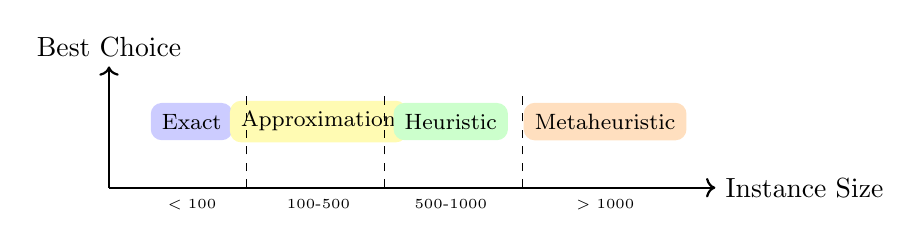
\begin{tikzpicture}[scale=0.7]
\draw[thick, ->] (0,0) -- (11,0) node[right] {Instance Size};
\draw[thick, ->] (0,0) -- (0,2.2) node[above] {Best Choice};
\node[fill=blue!20, rounded corners, inner sep=4pt] at (1.5,1.2) {\footnotesize Exact};
\node[fill=yellow!30, rounded corners, inner sep=4pt] at (3.8,1.2) {\footnotesize Approximation};
\node[fill=green!20, rounded corners, inner sep=4pt] at (6.2,1.2) {\footnotesize Heuristic};
\node[fill=orange!25, rounded corners, inner sep=4pt] at (9,1.2) {\footnotesize Metaheuristic};
\draw[dashed] (2.5,0) -- (2.5,1.8);
\draw[dashed] (5,0) -- (5,1.8);
\draw[dashed] (7.5,0) -- (7.5,1.8);
\node at (1.5,-0.3) {\tiny $<100$};
\node at (3.8,-0.3) {\tiny $100\text{-}500$};
\node at (6.2,-0.3) {\tiny $500\text{-}1000$};
\node at (9,-0.3) {\tiny $>1000$};
\end{tikzpicture}
\end{center}
\end{frame}

% =============================================================================
% SECTION 4: SELECTED ALGORITHMS
% =============================================================================
\section{Selected Algorithms}

\begin{frame}{Section 4: Algorithms We Implement}
\begin{center}
{\Large\textcolor{primaryblue}{\textbf{Maximum Marginal Return (MMR) and Genetic Algorithm (GA)}}}

\vspace{0.3cm}
{\normalsize Detailed algorithms with step-by-step examples}
\end{center}

\vspace{0.2cm}
\begin{columns}[t]
\column{0.48\textwidth}
\begin{block}{\textbf{MMR} -- Greedy Heuristic}
\begin{itemize}
    \item Fast: $O(W^2T)$ complexity
    \item Deterministic output
    \item Near-optimal ($<$5\% gap)
    \item \textbf{Ideal for real-time systems}
\end{itemize}
\end{block}

\column{0.48\textwidth}
\begin{alertblock}{\textbf{GA} -- Metaheuristic}
\begin{itemize}
    \item Flexible: $O(G \cdot P \cdot W \cdot T)$
    \item Population-based exploration
    \item Avoids local optima
    \item \textbf{Ideal for large instances}
\end{itemize}
\end{alertblock}
\end{columns}
\end{frame}

\begin{frame}{Why MMR + GA?}
\begin{columns}[t]
\column{0.48\textwidth}
\begin{block}{\textbf{Maximum Marginal Return (MMR)}}
\textbf{Why selected:}
\begin{itemize}
    \item \textcolor{accentgreen}{$O(W^2T)$} -- fastest complexity
    \item Simple to implement and verify
    \item Often near-optimal ($<$5\% gap)
    \item \textbf{Ideal for real-time missile defense}
\end{itemize}

\vspace{0.2cm}
\textbf{Key Formula:}
$$\Delta_{ij} = V_j \cdot q_j \cdot (1 - q_{ij})$$
{\small (Marginal reduction in survival)}
\end{block}

\column{0.48\textwidth}
\begin{alertblock}{\textbf{Genetic Algorithm (GA)}}
\textbf{Why selected:}
\begin{itemize}
    \item Population-based global search
    \item Natural selection drives optimization
    \item Well-studied for combinatorial problems
    \item \textbf{Effective for large instances ($>$100)}
    \item Easy to incorporate domain knowledge
\end{itemize}

\vspace{0.2cm}
\textbf{Key Idea:}

{\small Evolve population of solutions through selection, crossover, and mutation}
\end{alertblock}
\end{columns}

\vspace{0.3cm}
\begin{exampleblock}{Complementary Approaches}
\textbf{MMR} provides fast, deterministic baseline; \textbf{GA} performs global stochastic search across diverse solution space. Together, they represent greedy vs. evolutionary paradigms.
\end{exampleblock}
\end{frame}

% ===== MMR ALGORITHM =====
\begin{frame}{Algorithm 1: Maximum Marginal Return (MMR)}
\begin{block}{Core Idea}
\textbf{Greedy approach:} At each step, assign the unallocated weapon and target pair that yields the \textbf{maximum decrease} in survival value.
\end{block}

\vspace{0.2cm}
\begin{exampleblock}{Key Concepts}
\begin{itemize}
    \item \textbf{Tracking Value:} We track remaining survival value for each target.
    \item \textbf{Decrease Calculation:} $\text{decrease} = V[t] \times p[w][t]$
    \item \textbf{Value Update:} Once assigned, the target's value is permanently reduced:
    $$V[t] \gets V[t] - \text{decrease}$$
    \item \textbf{Iteration:} Repeat until all weapons are allocated.
\end{itemize}
\end{exampleblock}

\begin{alertblock}{Example: Diminishing Returns}
If T1 has $V=10$, W1 ($p=0.7$) yields decrease = 7.0.
New $V = 10 - 7 = 3.0$.
A second weapon W3 ($p=0.8$) on T1 now yields decrease = $3.0 \times 0.8 = 2.4$.
\end{alertblock}
\end{frame}

\begin{frame}[fragile]{MMR Algorithm: Pseudocode}
\begin{algorithm}[H]
\caption{Maximum Marginal Return (MMR) Algorithm}
\begin{algorithmic}[1]
\State $solution.Allocations \gets \emptyset$
\State $solution.Value \gets MaxValue$
\State $allocatedWeaponCount \gets 0$
\While{$allocatedWeaponCount \leq noOfWeapons$}
    \State $maxDecrease \gets MinValue$
    \State $k \gets 1$
    \While{$k \leq unallocatedWeapons.Count$}
        \State $i \gets 1$
        \While{$i \leq noOfTargets$}
            \State $decrease \gets targetValues[i] \times killProbabilities[i][k]$
            \If{$decrease > maxDecrease$}
                \State $maxDecrease \gets decrease$
                \State $allocatedTarget \gets i$
                \State $allocatedWeapon \gets k$
            \EndIf
            \State $i \gets i + 1$
        \EndWhile
        \State $k \gets k + 1$
    \EndWhile
    \State $unallocatedWeapons.Remove(allocatedWeapon)$
    \State $solution.Allocations[allocatedWeapon] \gets allocatedTarget$
    \State $targetValues[allocatedTarget] \gets targetValues[allocatedTarget] - maxDecrease$
    \State $allocatedWeaponCount \gets allocatedWeaponCount + 1$
\EndWhile
\State $solution.Value \gets \Call{CalculateSolutionValue}{solution.Allocations}$
\State \Return $solution$
\end{algorithmic}
\end{algorithm}
\end{frame}

\begin{frame}{MMR Example: Problem Setup (Naval Air Defense)}
\begin{columns}
\column{0.48\textwidth}
\textbf{Incoming Missiles (Targets):}
\begin{itemize}
    \item \textcolor{red}{T1}: Aircraft Carrier ($V=10$)
    \item \textcolor{orange}{T2}: Destroyer ($V=6$)
    \item \textcolor{yellow!80!black}{T3}: Supply Ship ($V=3$)
\end{itemize}

\vspace{0.3cm}
\textbf{Defensive Weapons:}
\begin{itemize}
    \item W1, W2, W3, W4 (4 interceptors)
\end{itemize}

\vspace{0.3cm}
\textbf{Goal:} Maximize expected damage prevented

\column{0.48\textwidth}
\textbf{Kill Probability Matrix $P_{ij}$:}
\begin{table}[h]
\centering
\small
\begin{tabular}{c|ccc}
     & T1 & T2 & T3 \\ \hline
W1 & 0.7 & 0.8 & 0.9 \\
W2 & 0.6 & 0.7 & 0.8 \\
W3 & 0.8 & 0.6 & 0.7 \\
W4 & 0.5 & 0.9 & 0.6 \\
\end{tabular}
\end{table}

\vspace{0.3cm}
\textbf{Objective Function:}
$$\text{Max } \sum_{j} V_j \times P_{kill,j}$$
\end{columns}
\end{frame}

\begin{frame}{MMR Iteration 1: Calculate Initial Marginal Returns}
\textbf{Algorithm Step:} Calculate marginal return for all weapon-target pairs

\vspace{0.2cm}
\textbf{Formula:} $MR_{ij} = V_j \times P_{ij}$ (since no weapons assigned yet)

\vspace{0.3cm}
\begin{table}[h]
\centering
\begin{tabular}{c|ccc}
\toprule
     & T1 ($V=10$) & T2 ($V=6$) & T3 ($V=3$) \\ \midrule
W1 & $10 \times 0.7 = 7.0$ & $6 \times 0.8 = 4.8$ & $3 \times 0.9 = 2.7$ \\
W2 & $10 \times 0.6 = 6.0$ & $6 \times 0.7 = 4.2$ & $3 \times 0.8 = 2.4$ \\
W3 & $10 \times 0.8 = \textcolor{red}{\textbf{8.0}}$ & $6 \times 0.6 = 3.6$ & $3 \times 0.7 = 2.1$ \\
W4 & $10 \times 0.5 = 5.0$ & $6 \times 0.9 = 5.4$ & $3 \times 0.6 = 1.8$ \\
\bottomrule
\end{tabular}
\end{table}

\begin{alertblock}{MMR Choice}
\textbf{Highest Marginal Return = 8.0} $\Rightarrow$ Assign \textbf{W3 $\rightarrow$ T1}
\end{alertblock}

\textbf{Current State:} T1: $P_{kill} = 0.8$, Expected = 8.0 \quad \textbf{Remaining:} W1, W2, W4
\end{frame}

\begin{frame}{MMR Iteration 2: Recalculate with Diminishing Returns}
\textbf{Algorithm Step:} Update marginal returns accounting for W3 already on T1

\vspace{0.2cm}
\textbf{For T1 (already has W3, $P_{kill} = 0.8$):}
\begin{itemize}
    \item W1: $P'_{kill} = 1-(0.3 \times 0.2) = 0.94$, $MR = 10(0.94-0.8) = 1.4$
    \item W2: $P'_{kill} = 1-(0.4 \times 0.2) = 0.92$, $MR = 10(0.92-0.8) = 1.2$
    \item W4: $P'_{kill} = 1-(0.5 \times 0.2) = 0.90$, $MR = 10(0.90-0.8) = 1.0$
\end{itemize}

\vspace{0.2cm}
\begin{table}[h]
\centering
\begin{tabular}{c|ccc}
\toprule
     & T1 (has W3) & T2 (empty) & T3 (empty) \\ \midrule
W1 & 1.4 & 4.8 & 2.7 \\
W2 & 1.2 & 4.2 & 2.4 \\
W4 & 1.0 & \textcolor{red}{\textbf{5.4}} & 1.8 \\
\bottomrule
\end{tabular}
\end{table}

\begin{alertblock}{MMR Choice}
\textbf{Highest Marginal Return = 5.4} $\Rightarrow$ Assign \textbf{W4 $\rightarrow$ T2}
\end{alertblock}

\textbf{Current State:} T1: 8.0, T2: $6 \times 0.9 = 5.4$ \quad \textbf{Total: 13.4}
\end{frame}

\begin{frame}{MMR Iterations 3 \& 4: Complete Assignment}
\textbf{Iteration 3:} Marginal returns for W1, W2

\begin{table}[h]
\centering
\begin{tabular}{c|ccc}
\toprule
     & T1 (has W3) & T2 (has W4) & T3 (empty) \\ \midrule
W1 & 1.4 & 0.48 & \textcolor{red}{\textbf{2.7}} \\
W2 & 1.2 & 0.42 & 2.4 \\
\bottomrule
\end{tabular}
\end{table}

$\Rightarrow$ Assign \textbf{W1 $\rightarrow$ T3} (MR = 2.7)

\vspace{0.3cm}
\textbf{Iteration 4:} Only W2 remains

\begin{table}[h]
\centering
\begin{tabular}{c|ccc}
\toprule
     & T1 (has W3) & T2 (has W4) & T3 (has W1) \\ \midrule
W2 & \textcolor{red}{\textbf{1.2}} & 0.42 & 0.24 \\
\bottomrule
\end{tabular}
\end{table}

$\Rightarrow$ Assign \textbf{W2 $\rightarrow$ T1} (MR = 1.2)

\begin{exampleblock}{Note: Diminishing Returns}
T3 with W1 has $P_{kill} = 0.9$, so adding W2: $P'_{kill} = 1-(0.2 \times 0.1) = 0.98$, $MR = 3(0.98-0.9) = 0.24$
\end{exampleblock}
\end{frame}

\begin{frame}{MMR: Final Solution}
\begin{center}
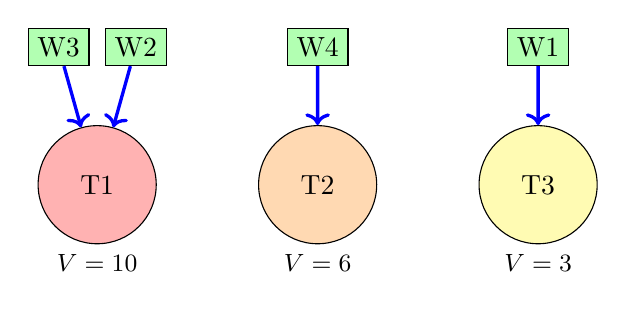
\begin{tikzpicture}[scale=0.7]
% Targets
\node[draw, circle, fill=red!30, minimum size=1.5cm] (T1) at (0,0) {T1};
\node[draw, circle, fill=orange!30, minimum size=1.5cm] (T2) at (4,0) {T2};
\node[draw, circle, fill=yellow!30, minimum size=1.5cm] (T3) at (8,0) {T3};

% Weapons assigned
\node[draw, rectangle, fill=green!30] (W3) at (-0.7,2.5) {W3};
\node[draw, rectangle, fill=green!30] (W2) at (0.7,2.5) {W2};
\node[draw, rectangle, fill=green!30] (W4) at (4,2.5) {W4};
\node[draw, rectangle, fill=green!30] (W1) at (8,2.5) {W1};

% Assignment arrows
\draw[->, very thick, blue] (W3) -- (T1);
\draw[->, very thick, blue] (W2) -- (T1);
\draw[->, very thick, blue] (W4) -- (T2);
\draw[->, very thick, blue] (W1) -- (T3);

% Labels
\node[below] at (T1.south) {\small $V=10$};
\node[below] at (T2.south) {\small $V=6$};
\node[below] at (T3.south) {\small $V=3$};
\end{tikzpicture}
\end{center}

\begin{block}{Final Assignment \& Expected Value}
\begin{itemize}
    \item \textbf{T1 (Aircraft Carrier):} W2, W3 $\rightarrow$ $P_{kill} = 1-(0.4 \times 0.2) = 0.92$, EV = $10 \times 0.92 = 9.2$
    \item \textbf{T2 (Destroyer):} W4 $\rightarrow$ $P_{kill} = 0.9$, EV = $6 \times 0.9 = 5.4$
    \item \textbf{T3 (Supply Ship):} W1 $\rightarrow$ $P_{kill} = 0.9$, EV = $3 \times 0.9 = 2.7$
\end{itemize}
\end{block}

\begin{alertblock}{Total Expected Value (Damage Prevented)}
$9.2 + 5.4 + 2.7 = \mathbf{17.3}$ \quad (out of max $10+6+3 = 19$)
\end{alertblock}
\end{frame}

\begin{frame}{MMR: Algorithm Analysis}
\begin{columns}[t]
\column{0.48\textwidth}
\begin{block}{Advantages}
\begin{itemize}
    \item \textbf{Fast:} $O(W^2 \cdot T)$ time complexity
    \item \textbf{Simple:} Easy to implement
    \item \textbf{Real-time capable:} Suitable for time-critical defense systems
    \item \textbf{Good results:} Often near-optimal
    \item \textbf{Adaptive:} Considers current state when making decisions
\end{itemize}
\end{block}

\column{0.48\textwidth}
\begin{alertblock}{Disadvantages}
\begin{itemize}
    \item \textbf{No optimality guarantee:} May miss globally optimal solution
    \item \textbf{Greedy nature:} Early decisions can't be reversed
    \item \textbf{Local optimization:} Focuses on immediate best choice
\end{itemize}
\end{alertblock}

\begin{exampleblock}{When to Use MMR}
\begin{itemize}
    \item Speed is critical
    \item Near-optimal is acceptable
    \item Real-time defense systems
    \item Large-scale problems
\end{itemize}
\end{exampleblock}
\end{columns}
\end{frame}

% ===== GENETIC ALGORITHM =====
\begin{frame}{Algorithm 2: Genetic Algorithm (GA)}
\begin{columns}[t]
\column{0.48\textwidth}
\begin{block}{Core Idea}
\textbf{Bio-inspired approach:} Evolve a population of candidate solutions through natural selection -- fitter individuals survive and reproduce.
\end{block}

\vspace{0.2cm}
\begin{center}
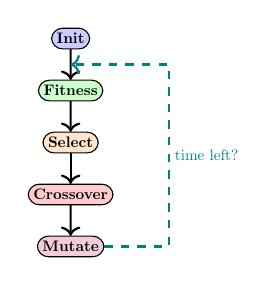
\begin{tikzpicture}[scale=0.55, transform shape]
\node[draw, rounded corners, fill=blue!20] (init) at (0,3.6) {\textbf{Init}};
\node[draw, rounded corners, fill=green!20] (eval) at (0,2.4) {\textbf{Fitness}};
\node[draw, rounded corners, fill=orange!20] (sel) at (0,1.2) {\textbf{Select}};
\node[draw, rounded corners, fill=red!20] (cross) at (0,0) {\textbf{Crossover}};
\node[draw, rounded corners, fill=purple!20] (mut) at (0,-1.2) {\textbf{Mutate}};
\draw[->, thick] (init) -- (eval);
\draw[->, thick] (eval) -- (sel);
\draw[->, thick] (sel) -- (cross);
\draw[->, thick] (cross) -- (mut);
\draw[->, thick, dashed, draw=teal] (mut.east) -- +(1.5,0) |- node[pos=0.25, right, text=teal] {time left?} (0, 3.0);
\end{tikzpicture}
\end{center}

\column{0.48\textwidth}
\begin{exampleblock}{GA for WTA}
\begin{itemize}
    \item \textbf{Chromosome Encoding:} \text{target assigned to weapon }$i$
    \item \textbf{Population Size:} $pop\_size = \max(W, T)$
    \item \textbf{Fitness:} $-Z$ (negative survival value; higher = better)
    \item \textbf{Selection:} Tournament ($k=3$)
    \item \textbf{Crossover:} Uniform ($p_{crossover} = 0.8$)
    \item \textbf{Mutation:} Random ($p_{mutation} = 1/W = 0.33$)
\end{itemize}
\end{exampleblock}

\begin{alertblock}{Key Advantage}
Explores \textbf{many solutions simultaneously} -- can escape local optima that trap greedy methods
\end{alertblock}
\end{columns}
\end{frame}

\begin{frame}[fragile]{GA: Encoding for WTA}
\begin{block}{Chromosome Representation}
Each individual (chromosome) is a vector of length $W$ (number of weapons):
$$\text{chromosome}[i] = j \quad \Rightarrow \quad \text{weapon } i \text{ assigned to target } j$$
\end{block}

\vspace{0.3cm}
\begin{center}
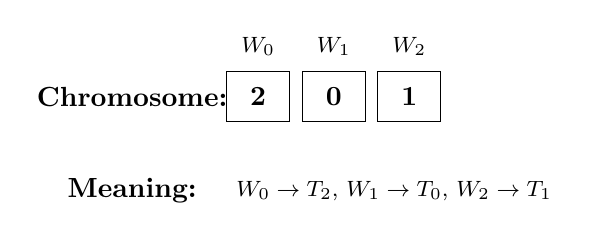
\begin{tikzpicture}[scale=0.8]
% Chromosome
\node at (-1.5, 0) {\textbf{Chromosome:}};
\draw (0, -0.4) rectangle (1, 0.4); \node at (0.5, 0) {\textbf{2}}; \node at (0.5, 0.8) {\footnotesize $W_0$};
\draw (1.2, -0.4) rectangle (2.2, 0.4); \node at (1.7, 0) {\textbf{0}}; \node at (1.7, 0.8) {\footnotesize $W_1$};
\draw (2.4, -0.4) rectangle (3.4, 0.4); \node at (2.9, 0) {\textbf{1}}; \node at (2.9, 0.8) {\footnotesize $W_2$};

% Meaning
\node at (-1.5, -1.5) {\textbf{Meaning:}};
\node[right] at (0, -1.5) {\footnotesize $W_0 \to T_2$, $W_1 \to T_0$, $W_2 \to T_1$};
\end{tikzpicture}
\end{center}

\vspace{0.3cm}
\begin{columns}[t]
\column{0.48\textwidth}
\begin{exampleblock}{Properties}
\begin{itemize}
    \item Fixed-length: always $W$ genes
    \item Each gene $\in \{0, 1, \ldots, T-1\}$
    \item Multiple weapons can target same target (many-to-one)
    \item Every weapon assigned to exactly one target
\end{itemize}
\end{exampleblock}

\column{0.48\textwidth}
\begin{alertblock}{Fitness Function (Survival Value $Z$)}
$$Z = \sum_{j=0}^{T-1} V_j \prod_{\substack{i: \text{chrom}[i]=j}} (1 - p_{ij})$$

Lower $Z$ = lower survival = \textbf{better} solution
\end{alertblock}
\end{columns}
\end{frame}

\begin{frame}[fragile]{GA Algorithm: Pseudocode}
\begin{algorithm}[H]
\caption{Genetic Algorithm}
\begin{algorithmic}[1]
\State $startTime \gets \text{Now}$
\State $endTime \gets startTime + allowedSearchTime$
\State $solution.Allocations \gets \emptyset$, \ \ $solution.Value \gets MaxValue$
\If{$noOfTargets > noOfWeapons$}
    \State $noOfIndividuals \gets noOfTargets$
\Else
    \State $noOfIndividuals \gets noOfWeapons$
\EndIf
\State $population \gets \Call{GenerateInitialPopulation}{noOfIndividuals}$
\While{$\text{Now} < endTime$}
    \State $individualNo \gets 1$
    \While{$individualNo \leq noOfIndividuals$}
        \State $solFromIndv \gets population[individualNo]$
        \State $solValue \gets \Call{CalculateSolutionValue}{solFromIndv}$
        \If{$solValue < solution.Value$}
            \State $solution \gets solFromIndv$
        \EndIf
        \State $individualNo \gets individualNo + 1$
    \EndWhile
    \State $parents \gets \Call{SelectParents}{population}$
    \State $population \gets \Call{CrossOver}{parents}$
    \State $population \gets \Call{Mutate}{population}$
\EndWhile
\State \Return $solution$
\end{algorithmic}
\end{algorithm}
\end{frame}

\begin{frame}{GA Example: Problem Setup (3 Weapons, 3 Targets)}
\begin{columns}
\column{0.48\textwidth}
\textbf{Targets (with strategic values):}
\begin{itemize}
    \item $T_0$: Value $V_0 = 10$
    \item $T_1$: Value $V_1 = 20$
    \item $T_2$: Value $V_2 = 30$
\end{itemize}

\vspace{0.3cm}
\textbf{Weapons:} $W_0, W_1, W_2$

\vspace{0.3cm}
\textbf{GA Parameters:}
\begin{itemize}
    \item Population size $= \max(3,3) = 3$
    \item Tournament $k = 3$, Crossover $= 0.8$
    \item Mutation rate $= 1/W = 1/3$
\end{itemize}

\column{0.48\textwidth}
\textbf{Kill Probability Matrix $p_{ij}$:}
\begin{table}[h]
\centering
\small
\begin{tabular}{c|ccc}
     & $T_0$ & $T_1$ & $T_2$ \\ \hline
$W_0$ & 0.3 & 0.2 & 0.1 \\
$W_1$ & 0.1 & 0.4 & 0.2 \\
$W_2$ & 0.2 & 0.3 & 0.5 \\
\end{tabular}
\end{table}

\vspace{0.3cm}
\textbf{Fitness (Survival Value $Z$):}
$$Z = \sum_{j} V_j \prod_{i: x_i=j} (1 - p_{ij})$$
{Lower $Z$ = better solution}
\end{columns}
\end{frame}

\begin{frame}{GA: Generation 0 -- Initialization \& Fitness}
\textbf{Three random individuals are generated:}

\vspace{0.3cm}
\begin{center}
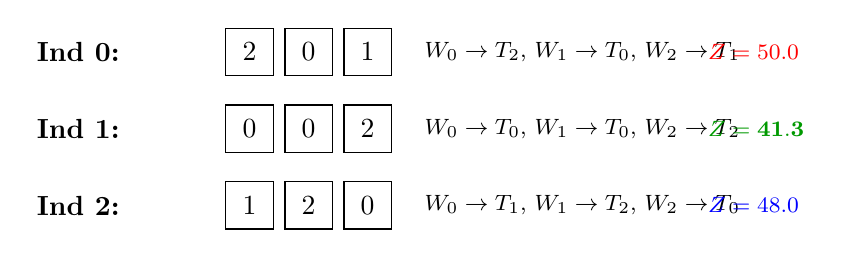
\begin{tikzpicture}[scale=0.75]
% Individual 0
\node at (-2.5, 3.2) {\textbf{Ind 0:}};
\draw (0, 2.8) rectangle (0.8, 3.6); \node at (0.4, 3.2) {2};
\draw (1.0, 2.8) rectangle (1.8, 3.6); \node at (1.4, 3.2) {0};
\draw (2.0, 2.8) rectangle (2.8, 3.6); \node at (2.4, 3.2) {1};
\node[right] at (3.2, 3.2) {\footnotesize $W_0 \to T_2$, $W_1 \to T_0$, $W_2 \to T_1$};
\node[right, red] at (8, 3.2) {\footnotesize $Z = 50.0$};

% Individual 1
\node at (-2.5, 1.9) {\textbf{Ind 1:}};
\draw (0, 1.5) rectangle (0.8, 2.3); \node at (0.4, 1.9) {0};
\draw (1.0, 1.5) rectangle (1.8, 2.3); \node at (1.4, 1.9) {0};
\draw (2.0, 1.5) rectangle (2.8, 2.3); \node at (2.4, 1.9) {2};
\node[right] at (3.2, 1.9) {\footnotesize $W_0 \to T_0$, $W_1 \to T_0$, $W_2 \to T_2$};
\node[right, green!60!black] at (8, 1.9) {\footnotesize $Z = \mathbf{41.3}$};

% Individual 2
\node at (-2.5, 0.6) {\textbf{Ind 2:}};
\draw (0, 0.2) rectangle (0.8, 1.0); \node at (0.4, 0.6) {1};
\draw (1.0, 0.2) rectangle (1.8, 1.0); \node at (1.4, 0.6) {2};
\draw (2.0, 0.2) rectangle (2.8, 1.0); \node at (2.4, 0.6) {0};
\node[right] at (3.2, 0.6) {\footnotesize $W_0 \to T_1$, $W_1 \to T_2$, $W_2 \to T_0$};
\node[right, blue] at (8, 0.6) {\footnotesize $Z = 48.0$};
\end{tikzpicture}
\end{center}

\vspace{0.2cm}
\begin{alertblock}{Detailed Fitness Calculation (Ind 1: $[0, 0, 2]$)}
\begin{itemize}
    \item $T_0$ attacked by $W_0, W_1$: $V_0 \times (1-0.3)(1-0.1) = 10 \times 0.7 \times 0.9 = 6.3$
    \item $T_1$ not attacked: $V_1 = 20.0$
    \item $T_2$ attacked by $W_2$: $V_2 \times (1-0.5) = 30 \times 0.5 = 15.0$
    \item $Z = 6.3 + 20.0 + 15.0 = \mathbf{41.3}$ \quad {\footnotesize (Best -- lowest survival)}
\end{itemize}
\end{alertblock}
\end{frame}

\begin{frame}{GA: Tournament Selection}
\begin{block}{Tournament Selection ($k = 3$)}
Randomly pick $k$ individuals from the population; select the one with \textbf{lowest $Z$} (best fitness).
\end{block}

\vspace{0.3cm}
\begin{center}
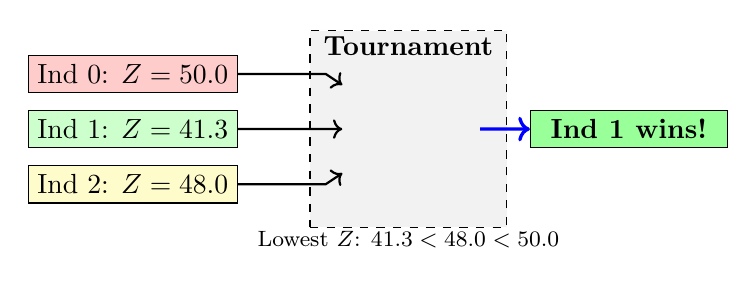
\begin{tikzpicture}[scale=0.7]
% Population
\node[draw, fill=red!20, minimum width=2.5cm] (i0) at (0, 3) {Ind 0: $Z = 50.0$};
\node[draw, fill=green!20, minimum width=2.5cm] (i1) at (0, 2) {Ind 1: $Z = 41.3$};
\node[draw, fill=yellow!20, minimum width=2.5cm] (i2) at (0, 1) {Ind 2: $Z = 48.0$};

% Tournament
\node[draw, dashed, fill=gray!10, minimum width=2.5cm, minimum height=2.5cm] at (5, 2) {};
\node at (5, 3.5) {\textbf{Tournament}};

\draw[->, thick] (i0.east) -- (3.5, 3) -- (3.8, 2.8);
\draw[->, thick] (i1.east) -- (3.5, 2) -- (3.8, 2);
\draw[->, thick] (i2.east) -- (3.5, 1) -- (3.8, 1.2);

% Winner
\node[draw, fill=green!40, minimum width=2.5cm] (winner) at (9, 2) {\textbf{Ind 1 wins!}};
\draw[->, very thick, blue] (6.3, 2) -- (winner.west);

\node at (5, 0) {\footnotesize Lowest $Z$: $41.3 < 48.0 < 50.0$};
\end{tikzpicture}
\end{center}

\vspace{0.2cm}
\begin{exampleblock}{Why Tournament Selection?}
\begin{itemize}
    \item \textbf{Selection pressure} adjustable via $k$: larger $k$ = stronger pressure
    \item Preserves \textbf{diversity}: weaker individuals still have a chance
    \item $O(k)$ per selection -- very efficient
\end{itemize}
\end{exampleblock}
\end{frame}

\begin{frame}{GA: Crossover \& Mutation}
\begin{block}{In This Example}
Both parents happen to be the same individual (Ind 1: $[0, 0, 2]$), so crossover produces an identical child. \textbf{Mutation} then introduces variation.
\end{block}

\vspace{0.2cm}
\begin{columns}[t]
\column{0.48\textwidth}
\begin{exampleblock}{Uniform Crossover}
$P_1 = [0, 0, 2]$, $P_2 = [0, 0, 2]$

\vspace{0.1cm}
Child (before mutation): $[0, 0, 2]$

\vspace{0.1cm}
{\footnotesize Identical parents $\Rightarrow$ identical child. Crossover preserves the best solution's genes.}
\end{exampleblock}

\column{0.48\textwidth}
\begin{alertblock}{Mutation (rate $= 1/3$)}
Each gene mutates with probability $1/3$:
\begin{itemize}
    \item Gene 0: rand $= 0.71 > 0.33$ $\Rightarrow$ \textbf{Keep} $0$
    \item Gene 1: rand $= 0.12 < 0.33$ $\Rightarrow$ \textbf{Mutate!} $0 \to 2$
    \item Gene 2: rand $= 0.55 > 0.33$ $\Rightarrow$ \textbf{Keep} $2$
\end{itemize}
\end{alertblock}
\end{columns}

\vspace{0.3cm}
\begin{center}
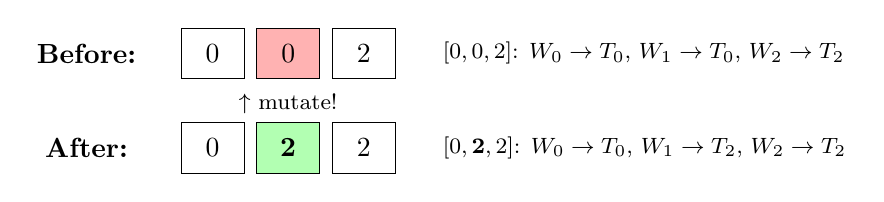
\begin{tikzpicture}[scale=0.8]
% Before
\node at (-1.5, 1) {\textbf{Before:}};
\draw[fill=white] (0, 0.6) rectangle (1, 1.4); \node at (0.5, 1) {0};
\draw[fill=red!30] (1.2, 0.6) rectangle (2.2, 1.4); \node at (1.7, 1) {0};
\draw[fill=white] (2.4, 0.6) rectangle (3.4, 1.4); \node at (2.9, 1) {2};
\node at (1.7, 0.2) {\footnotesize $\uparrow$ mutate!};

% After
\node at (-1.5, -0.5) {\textbf{After:}};
\draw[fill=white] (0, -0.9) rectangle (1, -0.1); \node at (0.5, -0.5) {0};
\draw[fill=green!30] (1.2, -0.9) rectangle (2.2, -0.1); \node at (1.7, -0.5) {\textbf{2}};
\draw[fill=white] (2.4, -0.9) rectangle (3.4, -0.1); \node at (2.9, -0.5) {2};

\node[right] at (4, 1) {\footnotesize $[0, 0, 2]$: $W_0 \to T_0$, $W_1 \to T_0$, $W_2 \to T_2$};
\node[right] at (4, -0.5) {\footnotesize $[0, \mathbf{2}, 2]$: $W_0 \to T_0$, $W_1 \to T_2$, $W_2 \to T_2$};
\end{tikzpicture}
\end{center}
\end{frame}

\begin{frame}{GA: Generation 1 -- Offspring Evaluation \& Replacement}
\begin{block}{Offspring Fitness: Child $C_1 = [0, 2, 2]$}
\begin{itemize}
    \item $T_0$ attacked by $W_0$: $V_0 \times (1-0.3) = 10 \times 0.7 = 7.0$
    \item $T_1$ not attacked: $V_1 = 20.0$
    \item $T_2$ attacked by $W_1, W_2$: $V_2 \times (1-0.2)(1-0.5) = 30 \times 0.8 \times 0.5 = 12.0$
    \item $Z = 7.0 + 20.0 + 12.0 = \mathbf{39.0}$ \quad {\footnotesize (Better than any parent!)}
\end{itemize}
\end{block}

\vspace{0.2cm}
\begin{alertblock}{Replacement: Child Replaces Worst Individual}
\begin{center}
\begin{tabular}{lccc}
\toprule
& \textbf{Before} & & \textbf{After} \\
\midrule
Ind 0 & $[2,0,1]$, $Z = 50.0$ & $\Rightarrow$ & \textcolor{green!60!black}{$[0,2,2]$, $Z = \mathbf{39.0}$} \\
Ind 1 & $[0,0,2]$, $Z = 41.3$ & $\Rightarrow$ & $[0,0,2]$, $Z = 41.3$ \\
Ind 2 & $[1,2,0]$, $Z = 48.0$ & $\Rightarrow$ & $[1,2,0]$, $Z = 48.0$ \\
\bottomrule
\end{tabular}
\end{center}
New best: $Z = 39.0$ (improved from 41.3)
\end{alertblock}

\vspace{0.2cm}
\begin{exampleblock}{Comparison with MMR on Same Problem}
MMR greedy gives $[0, 1, 2]$ with $Z = 10(0.7) + 20(0.6) + 30(0.5) = 7 + 12 + 15 = \mathbf{34.0}$

\vspace{0.1cm}
After 1 generation, GA (39.0) is still behind MMR (34.0) -- motivating \textbf{MMR-seeded initialization} in our Hybrid GA!
\end{exampleblock}
\end{frame}

\begin{frame}{GA: Parameters Summary}
\begin{block}{GA Configuration (Hasan \& Barua)}
All parameters follow the original paper implementation.
\end{block}

\vspace{0.3cm}
\begin{table}[h]
\centering
\begin{tabular}{lll}
\toprule
\textbf{Parameter} & \textbf{Value} & \textbf{Rationale} \\
\midrule
Population size & $\max(W, T)$ & Scales with problem size \\
Selection & Tournament ($k=3$) & Good selection pressure \\
Crossover rate & 0.8 & High recombination \\
Crossover type & Uniform & No positional bias \\
Mutation rate & $1/W$ & $\sim$1 gene per individual \\
Termination & Time-based & Fair comparison with MMR \\
\bottomrule
\end{tabular}
\end{table}

\vspace{0.2cm}
\begin{alertblock}{Time Budgets for Fair Comparison}
\begin{center}
\begin{tabular}{lc}
\toprule
\textbf{Problem Size} & \textbf{Time Budget} \\
\midrule
Small ($W \leq 30$) & 5 seconds \\
Medium ($W \leq 120$) & 20 seconds \\
Large ($W > 120$) & 60 seconds \\
\bottomrule
\end{tabular}
\end{center}
\end{alertblock}
\end{frame}

% =============================================================================
% SECTION 5: OUR MODIFICATIONS
% =============================================================================
\section{Our Modifications}

\begin{frame}{Section 5: Our Modifications}
\begin{center}
{\Large\textcolor{primaryblue}{\textbf{Improving MMR and GA with Novel Enhancements}}}

\vspace{0.5cm}
{\normalsize 3 modifications for each algorithm -- all designed by our team}
\end{center}

\vspace{0.3cm}
\begin{columns}[t]
\column{0.48\textwidth}
\begin{block}{MMR $\rightarrow$ MMR-IR}
\begin{enumerate}
    \item Tie-breaking by target value
    \item 1-opt local search
    \item 2-opt swap search
\end{enumerate}
{\small \textbf{Goal:} Escape greedy local optima}
\end{block}

\column{0.48\textwidth}
\begin{alertblock}{GA $\rightarrow$ Hybrid GA}
\begin{enumerate}
    \item MMR-seeded initialization
    \item Elitism + stagnation detection
    \item Threat-proportional mutation
\end{enumerate}
{\small \textbf{Goal:} Faster convergence + better exploration}
\end{alertblock}
\end{columns}
\end{frame}

% ===== MMR-IR MODIFICATIONS =====
\begin{frame}{Modification 1: MMR-IR (Iterative Refinement)}
\begin{block}{Overview: Three Enhancements to MMR}
The greedy MMR solution is a good starting point but may be suboptimal because early decisions cannot be reversed. Our modifications add \textbf{post-processing local search} to improve the greedy solution.
\end{block}

\vspace{0.3cm}
\begin{center}
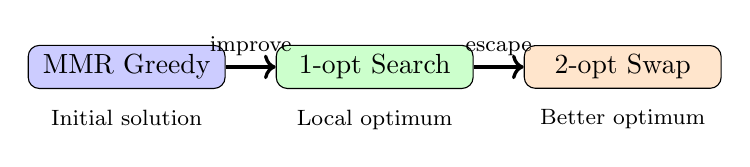
\begin{tikzpicture}[scale=0.7]
\node[draw, rounded corners, fill=blue!20, minimum width=2.5cm] (greedy) at (0,0) {MMR Greedy};
\node[draw, rounded corners, fill=green!20, minimum width=2.5cm] (opt1) at (4.5,0) {1-opt Search};
\node[draw, rounded corners, fill=orange!20, minimum width=2.5cm] (opt2) at (9,0) {2-opt Swap};
\draw[->, very thick] (greedy) -- node[above] {\footnotesize improve} (opt1);
\draw[->, very thick] (opt1) -- node[above] {\footnotesize escape} (opt2);

\node[below] at (0, -0.6) {\footnotesize Initial solution};
\node[below] at (4.5, -0.6) {\footnotesize Local optimum};
\node[below] at (9, -0.6) {\footnotesize Better optimum};
\end{tikzpicture}
\end{center}

\vspace{0.3cm}
\begin{exampleblock}{Enhancement 1: Tie-Breaking by Target Value}
When two weapon-target pairs have \textbf{equal marginal return}, prefer the pair targeting the \textbf{higher-value target}. This prioritizes coverage of critical targets.
\end{exampleblock}
\end{frame}

\begin{frame}{MMR-IR: 1-opt Local Search}
\begin{block}{Enhancement 2: 1-opt Incremental Local Search}
After MMR greedy completes, try \textbf{reassigning each weapon to every other target}. Accept if the objective improves. Repeat until no improvement found.
\end{block}

\vspace{0.2cm}
\begin{center}
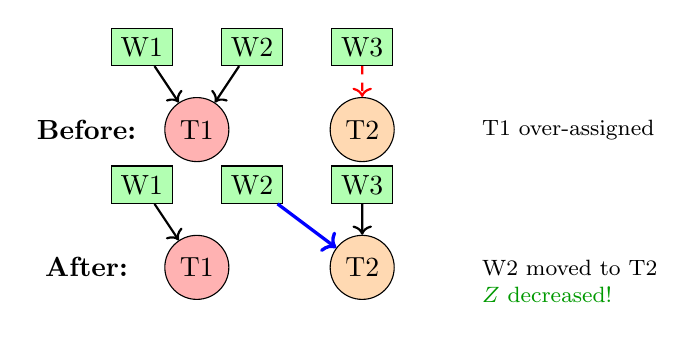
\begin{tikzpicture}[scale=0.7]
% Before
\node at (-1, 2.5) {\textbf{Before:}};
\node[draw, circle, fill=red!30] (T1a) at (1, 2.5) {T1};
\node[draw, circle, fill=orange!30] (T2a) at (4, 2.5) {T2};
\node[draw, rectangle, fill=green!30] (W1a) at (0, 4) {W1};
\node[draw, rectangle, fill=green!30] (W2a) at (2, 4) {W2};
\node[draw, rectangle, fill=green!30] (W3a) at (4, 4) {W3};
\draw[->, thick] (W1a) -- (T1a);
\draw[->, thick] (W2a) -- (T1a);
\draw[->, thick, red, dashed] (W3a) -- (T2a);

% After
\node at (-1, 0) {\textbf{After:}};
\node[draw, circle, fill=red!30] (T1b) at (1, 0) {T1};
\node[draw, circle, fill=orange!30] (T2b) at (4, 0) {T2};
\node[draw, rectangle, fill=green!30] (W1b) at (0, 1.5) {W1};
\node[draw, rectangle, fill=green!30] (W2b) at (2, 1.5) {W2};
\node[draw, rectangle, fill=green!30] (W3b) at (4, 1.5) {W3};
\draw[->, thick] (W1b) -- (T1b);
\draw[->, thick, blue, very thick] (W2b) -- (T2b);
\draw[->, thick] (W3b) -- (T2b);

\node[right] at (6, 2.5) {\footnotesize T1 over-assigned};
\node[right] at (6, 0) {\footnotesize W2 moved to T2};
\node[right, green!60!black] at (6, -0.5) {\footnotesize $Z$ decreased!};
\end{tikzpicture}
\end{center}

\begin{alertblock}{Incremental Evaluation}
Uses $O(1)$ delta computation per trial (survival array maintained via multiplication/division) instead of $O(WT)$ full recomputation. Max 20 passes until convergence.
\end{alertblock}
\end{frame}

\begin{frame}{MMR-IR: 2-opt Swap Search}
\begin{block}{Enhancement 3: 2-opt Swap Search}
After 1-opt converges, try \textbf{swapping the targets of two weapons simultaneously}. This can escape 1-opt local optima that single reassignments cannot.
\end{block}

\vspace{0.2cm}
\begin{center}
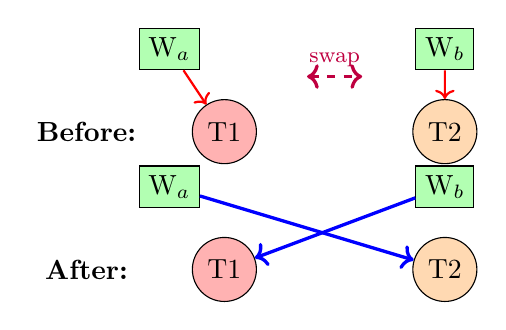
\begin{tikzpicture}[scale=0.7]
% Before
\node at (-1.5, 2.5) {\textbf{Before:}};
\node[draw, circle, fill=red!30] (T1) at (1, 2.5) {T1};
\node[draw, circle, fill=orange!30] (T2) at (5, 2.5) {T2};
\node[draw, rectangle, fill=green!30] (Wa) at (0, 4) {W$_a$};
\node[draw, rectangle, fill=green!30] (Wb) at (5, 4) {W$_b$};
\draw[->, thick, red] (Wa) -- (T1);
\draw[->, thick, red] (Wb) -- (T2);

% After
\node at (-1.5, 0) {\textbf{After:}};
\node[draw, circle, fill=red!30] (T1b) at (1, 0) {T1};
\node[draw, circle, fill=orange!30] (T2b) at (5, 0) {T2};
\node[draw, rectangle, fill=green!30] (Wab) at (0, 1.5) {W$_a$};
\node[draw, rectangle, fill=green!30] (Wbb) at (5, 1.5) {W$_b$};
\draw[->, thick, blue, very thick] (Wab) -- (T2b);
\draw[->, thick, blue, very thick] (Wbb) -- (T1b);

% Swap arrow
\draw[<->, very thick, purple, dashed] (2.5, 3.5) -- (3.5, 3.5);
\node[above, purple] at (3, 3.5) {\footnotesize swap};
\end{tikzpicture}
\end{center}

\begin{exampleblock}{Why 2-opt Helps}
\begin{itemize}
    \item 1-opt is stuck: moving W$_a$ alone worsens T1, moving W$_b$ alone worsens T2
    \item But swapping \textbf{both simultaneously} can improve the total objective
    \item Max 3 passes to limit runtime; incremental $O(1)$ delta per trial
\end{itemize}
\end{exampleblock}
\end{frame}

% ===== HYBRID GA MODIFICATIONS =====
\begin{frame}{Modification 2: Hybrid GA -- Overview}
\begin{block}{Three Weaknesses of Standard GA on WTA}
\begin{enumerate}
    \item \textbf{Random initialization} -- in high-dimensional space ($W \times T$ variables), random solutions are far from optimal
    \item \textbf{No elitism} -- the best solution found can be \textbf{lost} when replaced by offspring
    \item \textbf{Blind mutation} -- random target reassignment ignores which targets \textbf{need} more weapons
\end{enumerate}
\end{block}

\vspace{0.3cm}
\begin{alertblock}{Our Three Fixes}
\begin{center}
\begin{tabular}{lll}
\toprule
\textbf{Weakness} & \textbf{Our Fix} & \textbf{Type} \\
\midrule
Random initialization & MMR-seeded init & Warm start \\
No elitism / stagnation & Elitism + detection & Preservation \\
Blind mutation & Threat-proportional & \textbf{WTA-specific} \\
\bottomrule
\end{tabular}
\end{center}
\end{alertblock}
\end{frame}

\begin{frame}[fragile]{Hybrid GA Mod 1: MMR-Seeded Initialization}
\begin{block}{Idea: Start from a Good Solution}
Instead of initializing \textbf{all} individuals randomly, seed \texttt{population[0]} with the MMR greedy solution. The rest remain random for diversity.
\end{block}

\vspace{0.3cm}
\begin{center}
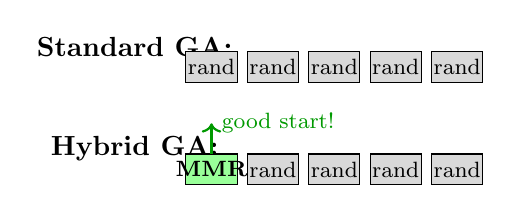
\begin{tikzpicture}[scale=0.65]
% Standard GA
\node at (-1, 3.5) {\textbf{Standard GA:}};
\foreach \i in {0,...,4} {
    \draw[fill=gray!30] (\i*1.2, 2.8) rectangle (\i*1.2+1, 3.4);
    \node at (\i*1.2+0.5, 3.1) {\footnotesize rand};
}

% Hybrid GA
\node at (-1, 1.5) {\textbf{Hybrid GA:}};
\draw[fill=green!40] (0, 0.8) rectangle (1, 1.4);
\node at (0.5, 1.1) {\footnotesize \textbf{MMR}};
\foreach \i in {1,...,4} {
    \draw[fill=gray!30] (\i*1.2, 0.8) rectangle (\i*1.2+1, 1.4);
    \node at (\i*1.2+0.5, 1.1) {\footnotesize rand};
}

% Arrow
\draw[->, thick, green!60!black] (0.5, 1.4) -- (0.5, 2) node[right] {\footnotesize good start!};
\end{tikzpicture}
\end{center}

\begin{exampleblock}{Why This Works}
\begin{itemize}
    \item MMR gives a \textbf{near-optimal} starting point in $O(W^2T)$ time
    \item GA then \textbf{refines} this solution via crossover and mutation
    \item Random individuals provide \textbf{genetic diversity} to avoid local optima
    \item For large instances ($W=375$), this saves hundreds of wasted generations
\end{itemize}
\end{exampleblock}
\end{frame}

\begin{frame}{Hybrid GA Mod 2: Elitism + Stagnation Detection}
\begin{block}{Idea: Never Lose the Best, Re-diversify When Stuck}
\begin{itemize}
    \item \textbf{Elitism:} Preserve top 10\% of population each generation (directly copied to next generation without modification)
    \item \textbf{Stagnation detection:} If best fitness unchanged for 5 consecutive generations, inject fresh random individuals to re-diversify
\end{itemize}
\end{block}

\vspace{0.2cm}
\begin{center}
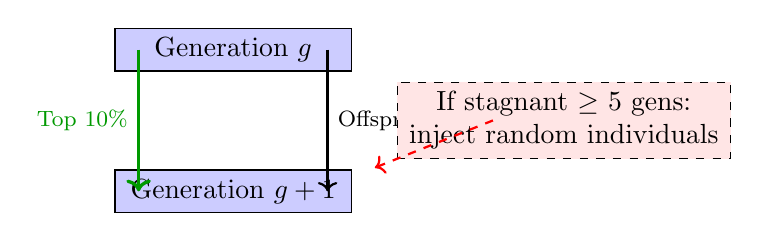
\begin{tikzpicture}[scale=0.6]
% Generation flow
\node[draw, fill=blue!20, minimum width=3cm] (gen1) at (0, 3) {Generation $g$};
\node[draw, fill=blue!20, minimum width=3cm] (gen2) at (0, 0) {Generation $g+1$};

% Elite arrow
\draw[->, very thick, green!60!black] (-2, 3) -- (-2, 0) node[midway, left] {\footnotesize Top 10\%};

% Offspring arrow
\draw[->, thick] (2, 3) -- (2, 0) node[midway, right] {\footnotesize Offspring (90\%)};

% Stagnation
\node[draw, dashed, fill=red!10, text width=4cm, align=center] at (7, 1.5) {If stagnant $\geq$ 5 gens:\\ inject random individuals};
\draw[->, thick, red, dashed] (5.5, 1.5) -- (3, 0.5);
\end{tikzpicture}
\end{center}

\begin{alertblock}{Without Elitism (Standard GA)}
A good solution in generation $g$ can be completely lost if all offspring are worse. This is especially problematic with small time budgets.
\end{alertblock}
\end{frame}

\begin{frame}{Hybrid GA Mod 3: Threat-Proportional Mutation}
\begin{block}{Idea: Domain-Aware Mutation (Novel, WTA-Specific)}
Instead of mutating to a \textbf{uniformly random} target, bias mutation toward targets with \textbf{high remaining threat}:
$$\text{remaining\_threat}[j] = V_j \times \prod_{i: x_i = j} (1 - p_{ij})$$

\textbf{Mutation target selection:} $P(\text{mutate to } j) \propto \text{remaining\_threat}[j]$
\end{block}

\vspace{0.2cm}
\begin{columns}[t]
\column{0.48\textwidth}
\begin{exampleblock}{Standard Mutation}
\begin{itemize}
    \item Pick random target uniformly
    \item May reassign to already well-covered target (wasted mutation)
    \item No domain knowledge used
\end{itemize}
\end{exampleblock}

\column{0.48\textwidth}
\begin{alertblock}{Threat-Proportional Mutation}
\begin{itemize}
    \item High-value, poorly-covered targets get more mutations
    \item Focuses search where improvement is \textbf{most needed}
    \item \textbf{Novel:} This is our original WTA-specific contribution
\end{itemize}
\end{alertblock}
\end{columns}

\vspace{0.2cm}
\begin{block}{Example}
If T1 ($V=100$, survival=0.6) and T2 ($V=20$, survival=0.1): \\
threat$_1 = 100 \times 0.6 = 60$, threat$_2 = 20 \times 0.1 = 2$ \\
$\Rightarrow$ T1 is 30$\times$ more likely to receive a mutated weapon than T2
\end{block}
\end{frame}

\begin{frame}{Hybrid GA: Modifications Summary}
\begin{center}
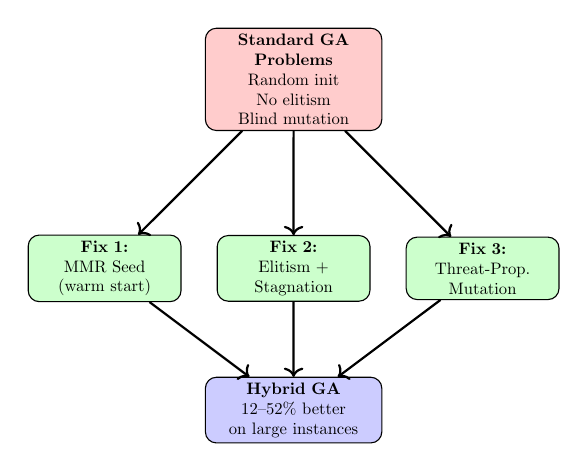
\begin{tikzpicture}[scale=0.6, transform shape]
\node[draw, rounded corners, fill=red!20, text width=3.5cm, align=center] (problem) at (0, 4) {\textbf{Standard GA Problems}\\Random init\\No elitism\\Blind mutation};

\node[draw, rounded corners, fill=green!20, text width=3cm, align=center] (fix1) at (-4, 0) {\textbf{Fix 1:}\\MMR Seed\\(warm start)};
\node[draw, rounded corners, fill=green!20, text width=3cm, align=center] (fix2) at (0, 0) {\textbf{Fix 2:}\\Elitism +\\Stagnation};
\node[draw, rounded corners, fill=green!20, text width=3cm, align=center] (fix3) at (4, 0) {\textbf{Fix 3:}\\Threat-Prop.\\Mutation};

\node[draw, rounded corners, fill=blue!20, text width=3.5cm, align=center] (result) at (0, -3) {\textbf{Hybrid GA}\\12--52\% better\\on large instances};

\draw[->, thick] (problem) -- (fix1);
\draw[->, thick] (problem) -- (fix2);
\draw[->, thick] (problem) -- (fix3);
\draw[->, thick] (fix1) -- (result);
\draw[->, thick] (fix2) -- (result);
\draw[->, thick] (fix3) -- (result);
\end{tikzpicture}
\end{center}

\begin{alertblock}{Key Insight}
Each modification targets a \textbf{specific weakness}. Together, they transform a struggling standard GA into a competitive solver that matches or beats MMR on all problem sizes.
\end{alertblock}
\end{frame}

% =============================================================================
% SECTION 6: EXPERIMENTAL SETUP
% =============================================================================
\section{Experiments \& Results}

\begin{frame}{Section 6: Experimental Setup}
\begin{center}
{\Large\textcolor{primaryblue}{\textbf{Dataset Design, Setup, and Results}}}

\vspace{0.5cm}
{\normalsize 180 instances, 4 algorithms, 9 categories}
\end{center}
\end{frame}

\begin{frame}{Dataset Design: Custom Synthetic Benchmark}
\begin{block}{Why Design Our Own Dataset?}
We created a synthetic dataset to systematically test \textbf{scaling behavior} across two dimensions: \textbf{problem size} (small/medium/large) and \textbf{resource availability} (balanced/scarce/rich).
\end{block}

\vspace{0.2cm}
\begin{table}[h]
\centering
\small
\begin{tabular}{llccc}
\toprule
\textbf{Tier} & \textbf{Scenario} & \textbf{Weapons ($W$)} & \textbf{Targets ($T$)} & \textbf{Instances} \\
\midrule
Small & Balanced ($W = T$) & 20 & 20 & 20 \\
Small & Scarce ($W < T$) & 10 & 20 & 20 \\
Small & Rich ($W > T$) & 30 & 20 & 20 \\
\midrule
Medium & Balanced & 100 & 100 & 20 \\
Medium & Scarce & 50 & 100 & 20 \\
Medium & Rich & 150 & 100 & 20 \\
\midrule
Large & Balanced & 250 & 250 & 20 \\
Large & Scarce & 125 & 250 & 20 \\
Large & Rich & 375 & 250 & 20 \\
\bottomrule
\end{tabular}
\end{table}

\begin{center}
\textbf{Total: 180 instances} (9 categories $\times$ 20 instances each)
\end{center}
\end{frame}

\begin{frame}{Dataset Parameters and Scenarios}
\begin{columns}[t]
\column{0.48\textwidth}
\begin{block}{Instance Parameters}
\begin{itemize}
    \item \textbf{Target values:} $V_j \sim U(10, 100)$ integers
    \item \textbf{Kill probabilities:} $p_{ij} \sim U(0.05, 0.90)$
    \item \textbf{RNG seed:} 42 (reproducible)
    \item \textbf{Format:} JSON files
\end{itemize}
\end{block}

\begin{exampleblock}{Statistical Testing}
\begin{itemize}
    \item \textbf{Wilcoxon signed-rank test} ($\alpha = 0.05$) for pairwise algorithm comparison
    \item 20 instances per category ensures statistical validity
\end{itemize}
\end{exampleblock}

\column{0.48\textwidth}
\begin{alertblock}{Scenario Rationale}
\textbf{Balanced} ($W = T$): Standard benchmark; each weapon covers one target on average.

\vspace{0.2cm}
\textbf{Scarce} ($W < T$): Hardest scenario; not enough weapons for all targets. Unengaged targets have 100\% survival.

\vspace{0.2cm}
\textbf{Rich} ($W > T$): Easiest scenario; surplus weapons allow thorough coverage. Lower objective values expected.
\end{alertblock}
\end{columns}
\end{frame}

\begin{frame}{Algorithms Compared}
\begin{table}[h]
\centering
\begin{tabular}{lp{5cm}l}
\toprule
\textbf{Algorithm} & \textbf{Description} & \textbf{Type} \\
\midrule
\textbf{MMR (orig)} & Maximum Marginal Return greedy heuristic. Faithful implementation from Hasan \& Barua. & Heuristic \\
\addlinespace
\textbf{MMR-IR (mod)} & MMR + tie-breaking + 1-opt local search + 2-opt swap search. & Enhanced Heuristic \\
\addlinespace
\textbf{GA (orig)} & Standard Genetic Algorithm. Faithful implementation from Hasan \& Barua. & Metaheuristic \\
\addlinespace
\textbf{Hybrid GA (mod)} & GA + MMR seed + elitism + stagnation detection + threat-proportional mutation. & Enhanced Meta. \\
\bottomrule
\end{tabular}
\end{table}

\begin{block}{Fair Comparison}
All algorithms run on the \textbf{same instances} with \textbf{same time budgets}. GA variants use identical time limits. Results measured as \textbf{expected survival value} $Z$ (lower = better).
\end{block}
\end{frame}

% =============================================================================
% RESULTS
% =============================================================================

\begin{frame}{Results: Solution Quality -- Box Plots}
\begin{center}
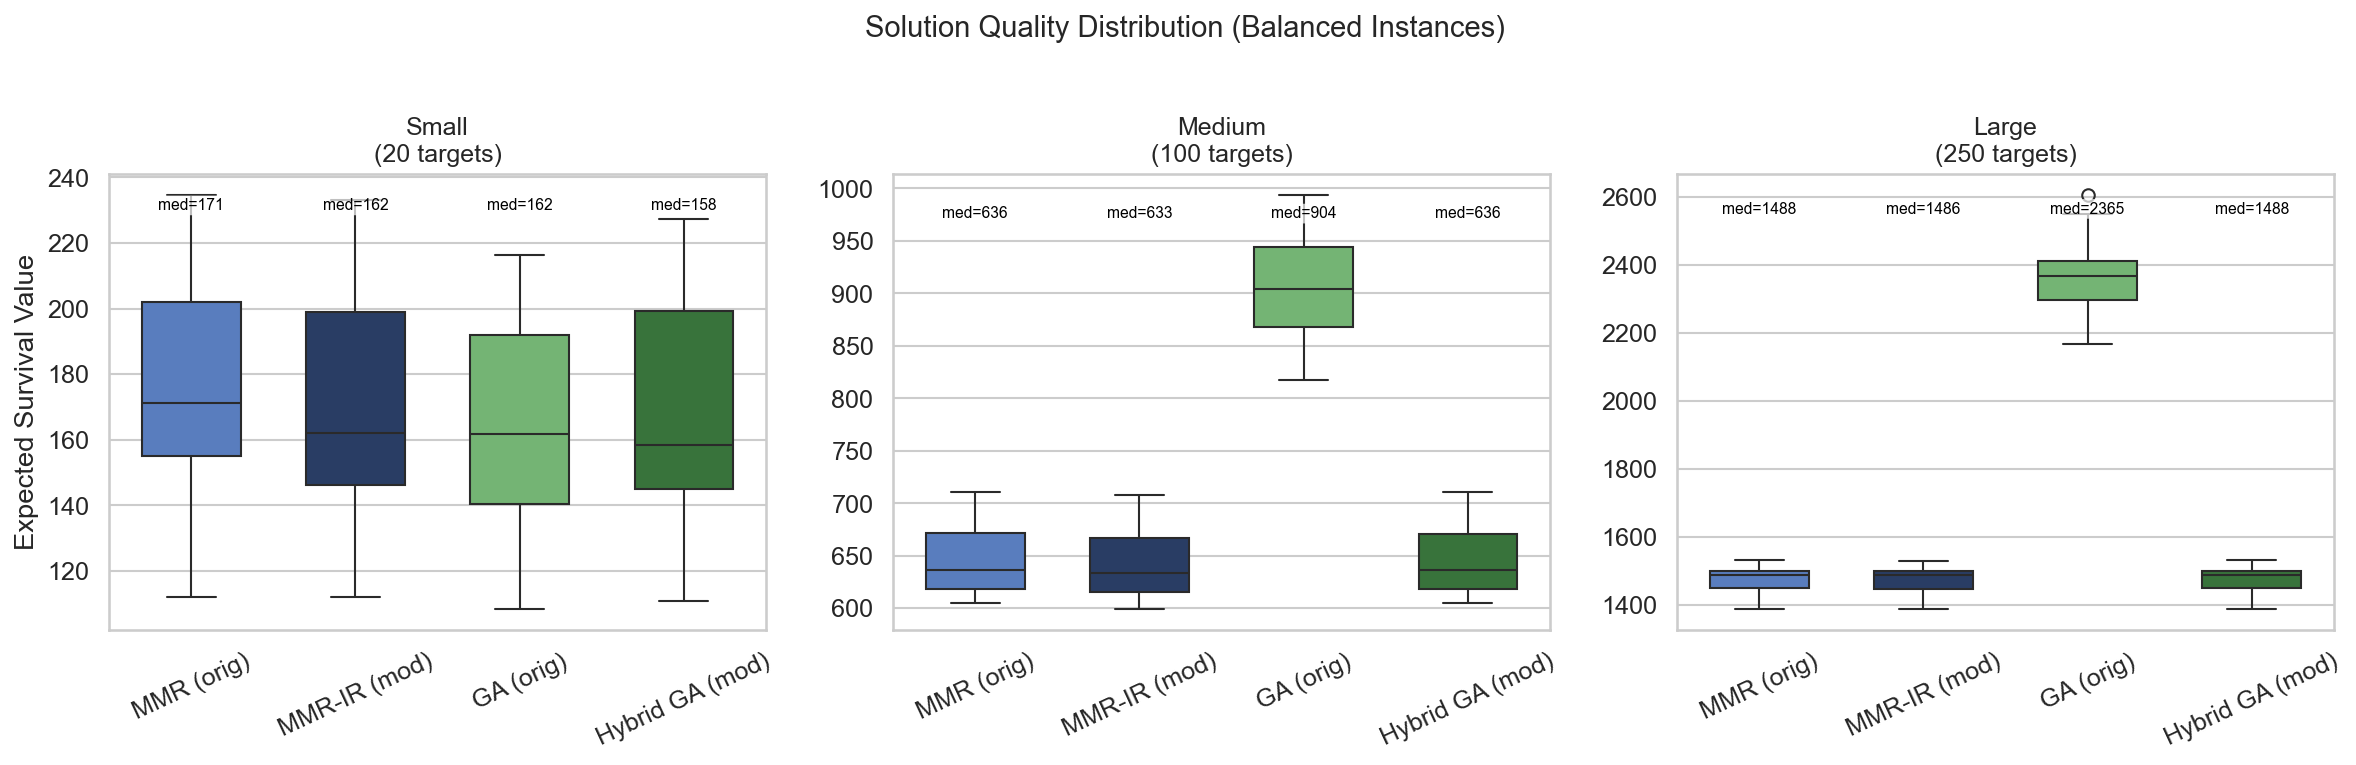
\includegraphics[width=0.92\textwidth]{images/01_box_solution_quality.png}
\end{center}

\vspace{-0.2cm}
{\footnotesize Box plots show distribution of objective values (lower = better) across balanced instances per tier.}
\end{frame}

\begin{frame}{Results: Mean Objective Value by Tier}
\begin{center}
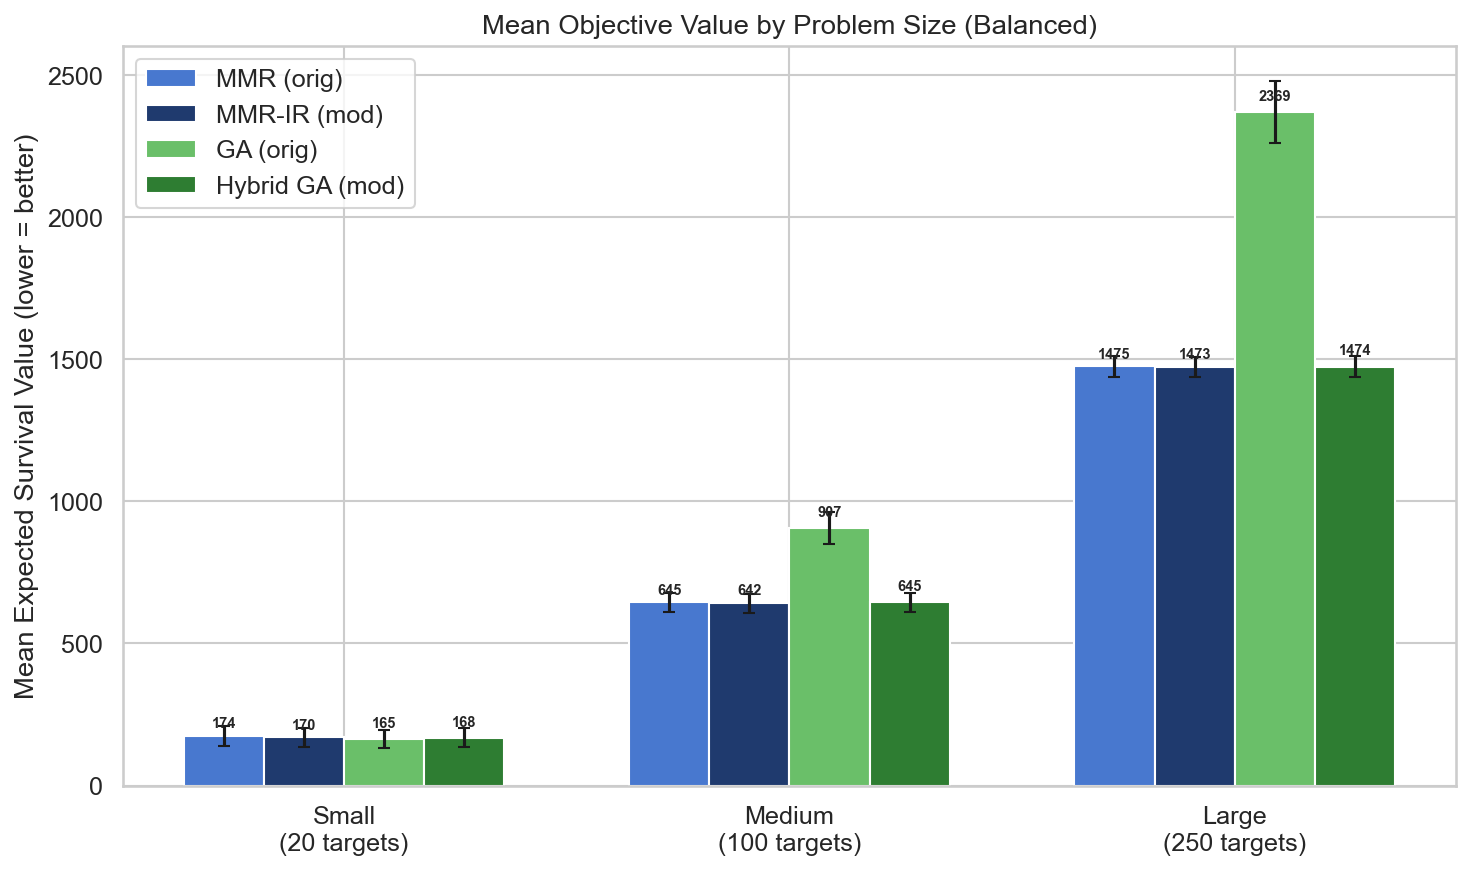
\includegraphics[width=0.92\textwidth]{images/02_bar_mean_objective.png}
\end{center}

\vspace{-0.2cm}
{\footnotesize GA (orig) falls dramatically behind on medium and large tiers due to random initialization + no elitism.}
\end{frame}

\begin{frame}{Results: Improvement of Modifications}
\begin{center}
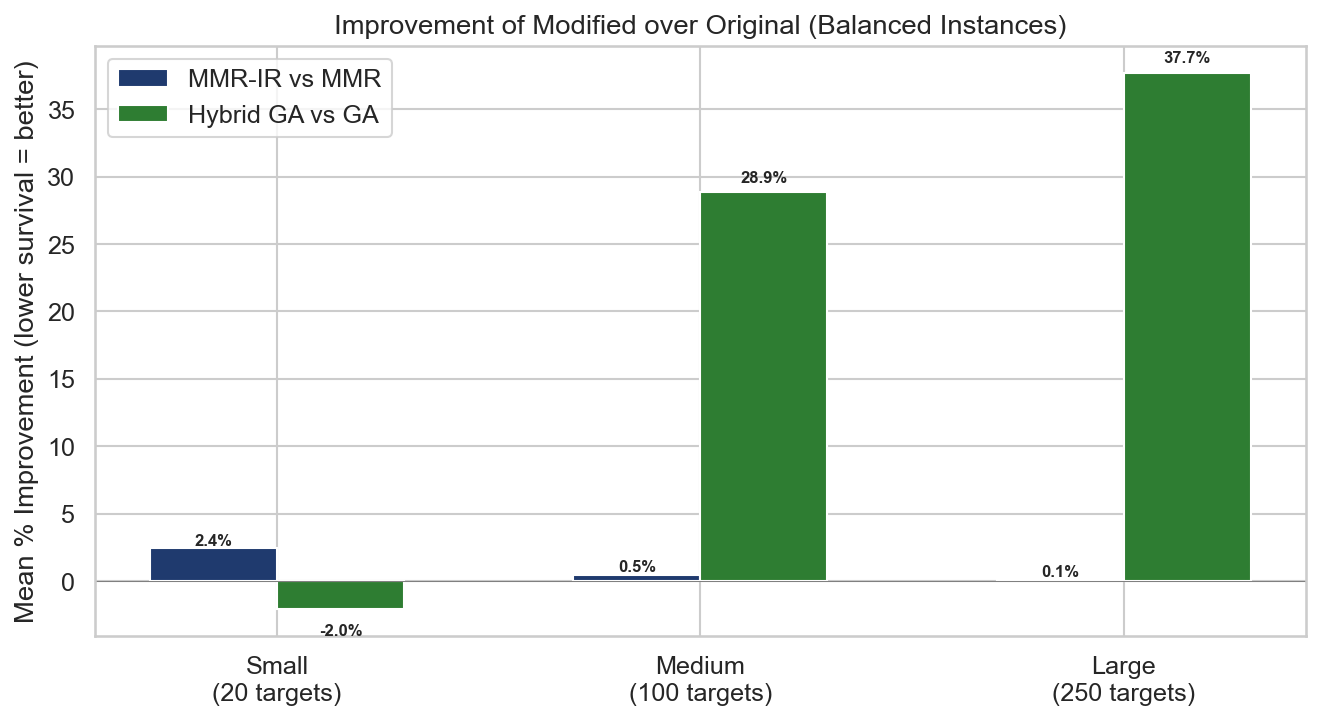
\includegraphics[width=0.92\textwidth]{images/03_bar_improvement.png}
\end{center}

\vspace{-0.2cm}
{\footnotesize Percentage improvement of modified algorithms over their original counterparts. GA improvement grows with problem size.}
\end{frame}

\begin{frame}{Results: Runtime Scalability}
\begin{center}
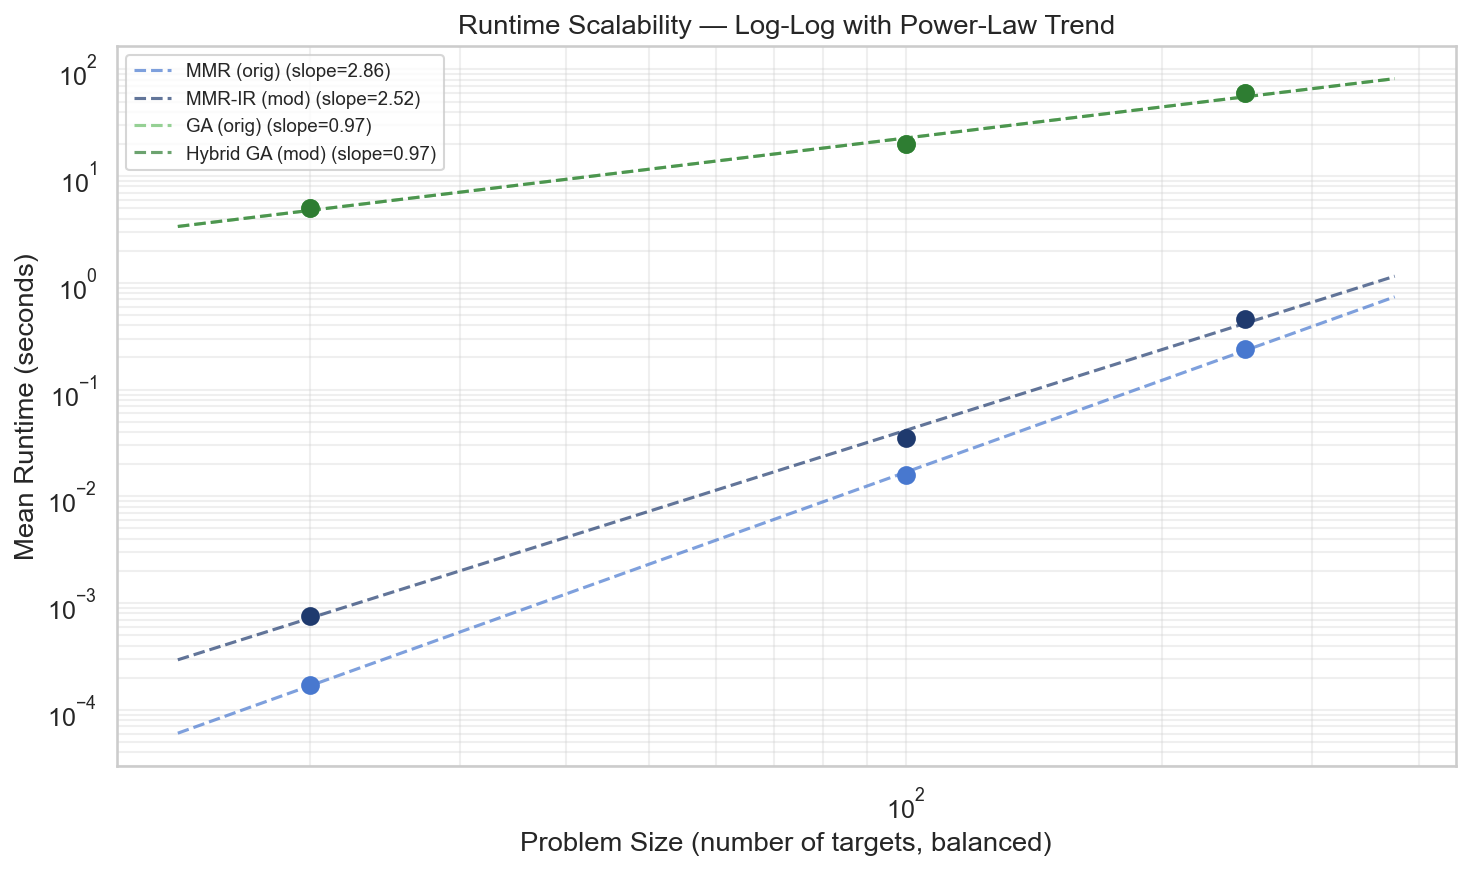
\includegraphics[width=0.92\textwidth]{images/04_line_time_scalability.png}
\end{center}

\vspace{-0.2cm}
{\footnotesize Log-log scale. MMR variants are orders of magnitude faster. GA variants use their full time budget.}
\end{frame}

\begin{frame}{Results: Optimality Gap}
\begin{center}
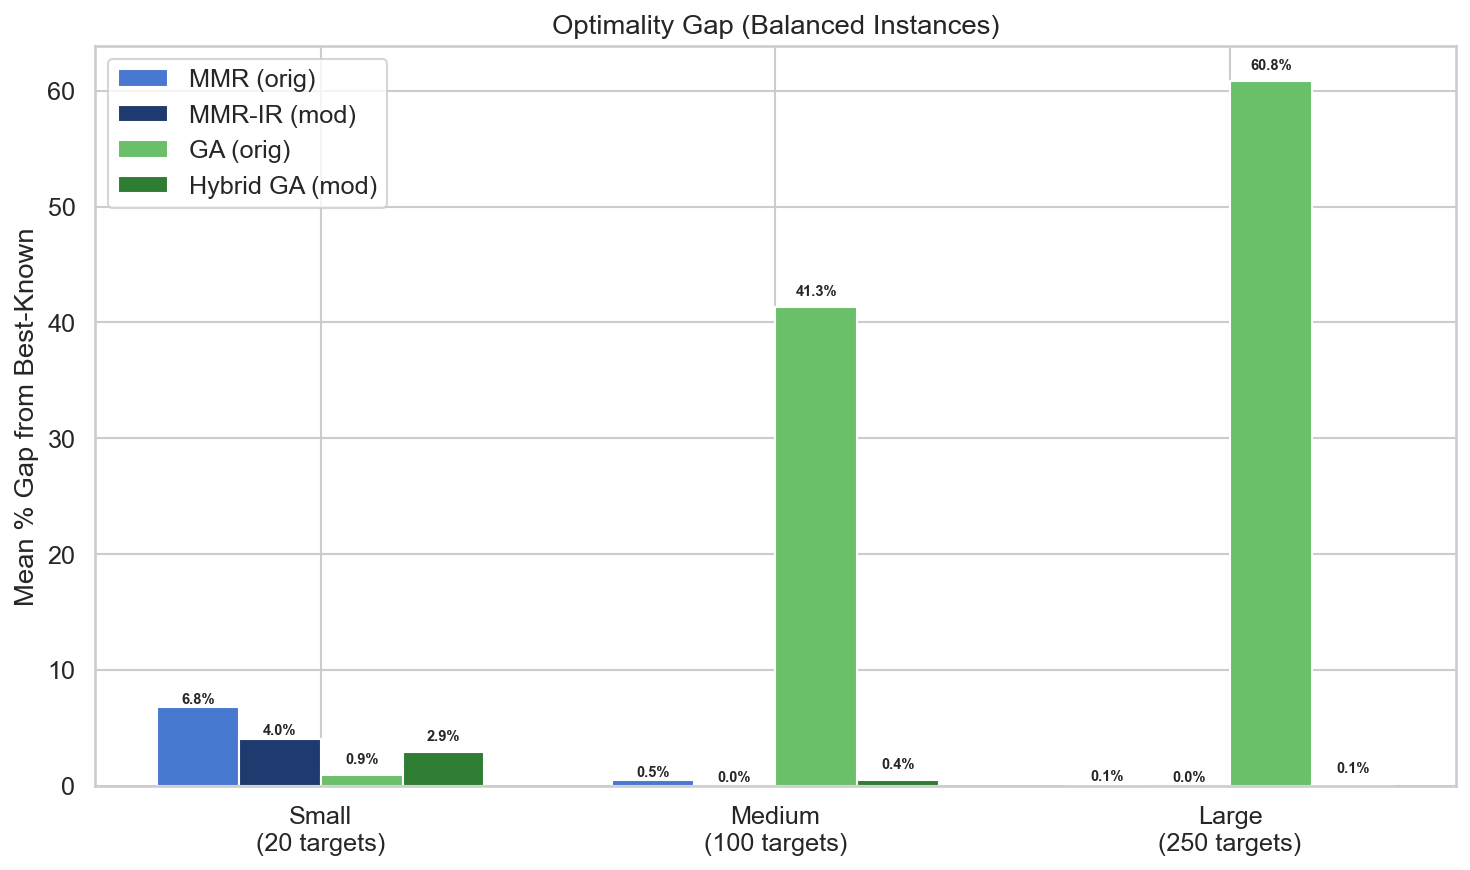
\includegraphics[width=0.92\textwidth]{images/05_bar_gap.png}
\end{center}

\vspace{-0.2cm}
{\footnotesize Gap from best-known solution. GA (orig) has the largest gap, especially on large instances.}
\end{frame}

\begin{frame}{Results: Scenario Comparison}
\begin{center}
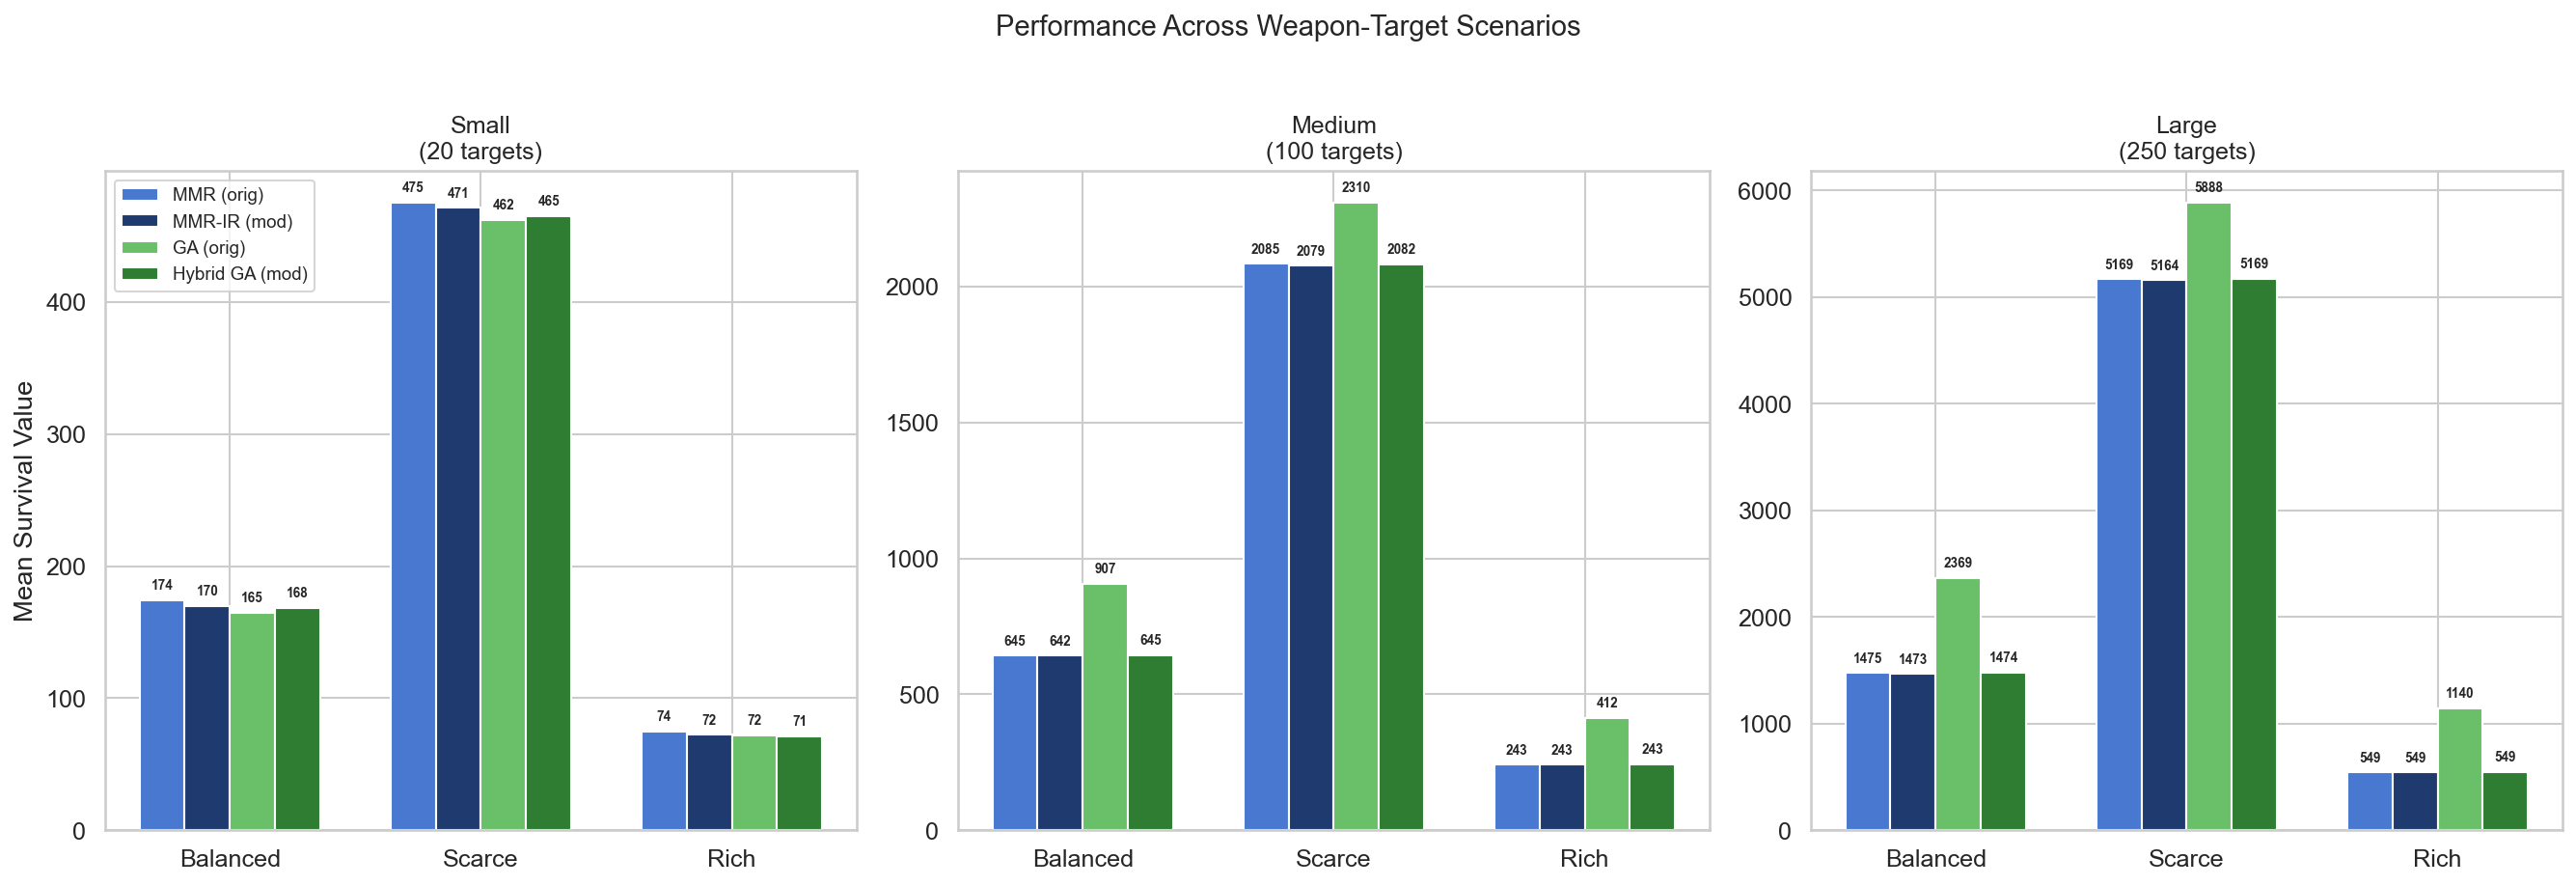
\includegraphics[width=0.92\textwidth]{images/06_scenario_comparison.png}
\end{center}

\vspace{-0.2cm}
{\footnotesize Performance across balanced, scarce, and rich scenarios. Scarce has highest objective (hardest), rich has lowest (easiest).}
\end{frame}

\begin{frame}{Results: Value Distributions}
\begin{center}
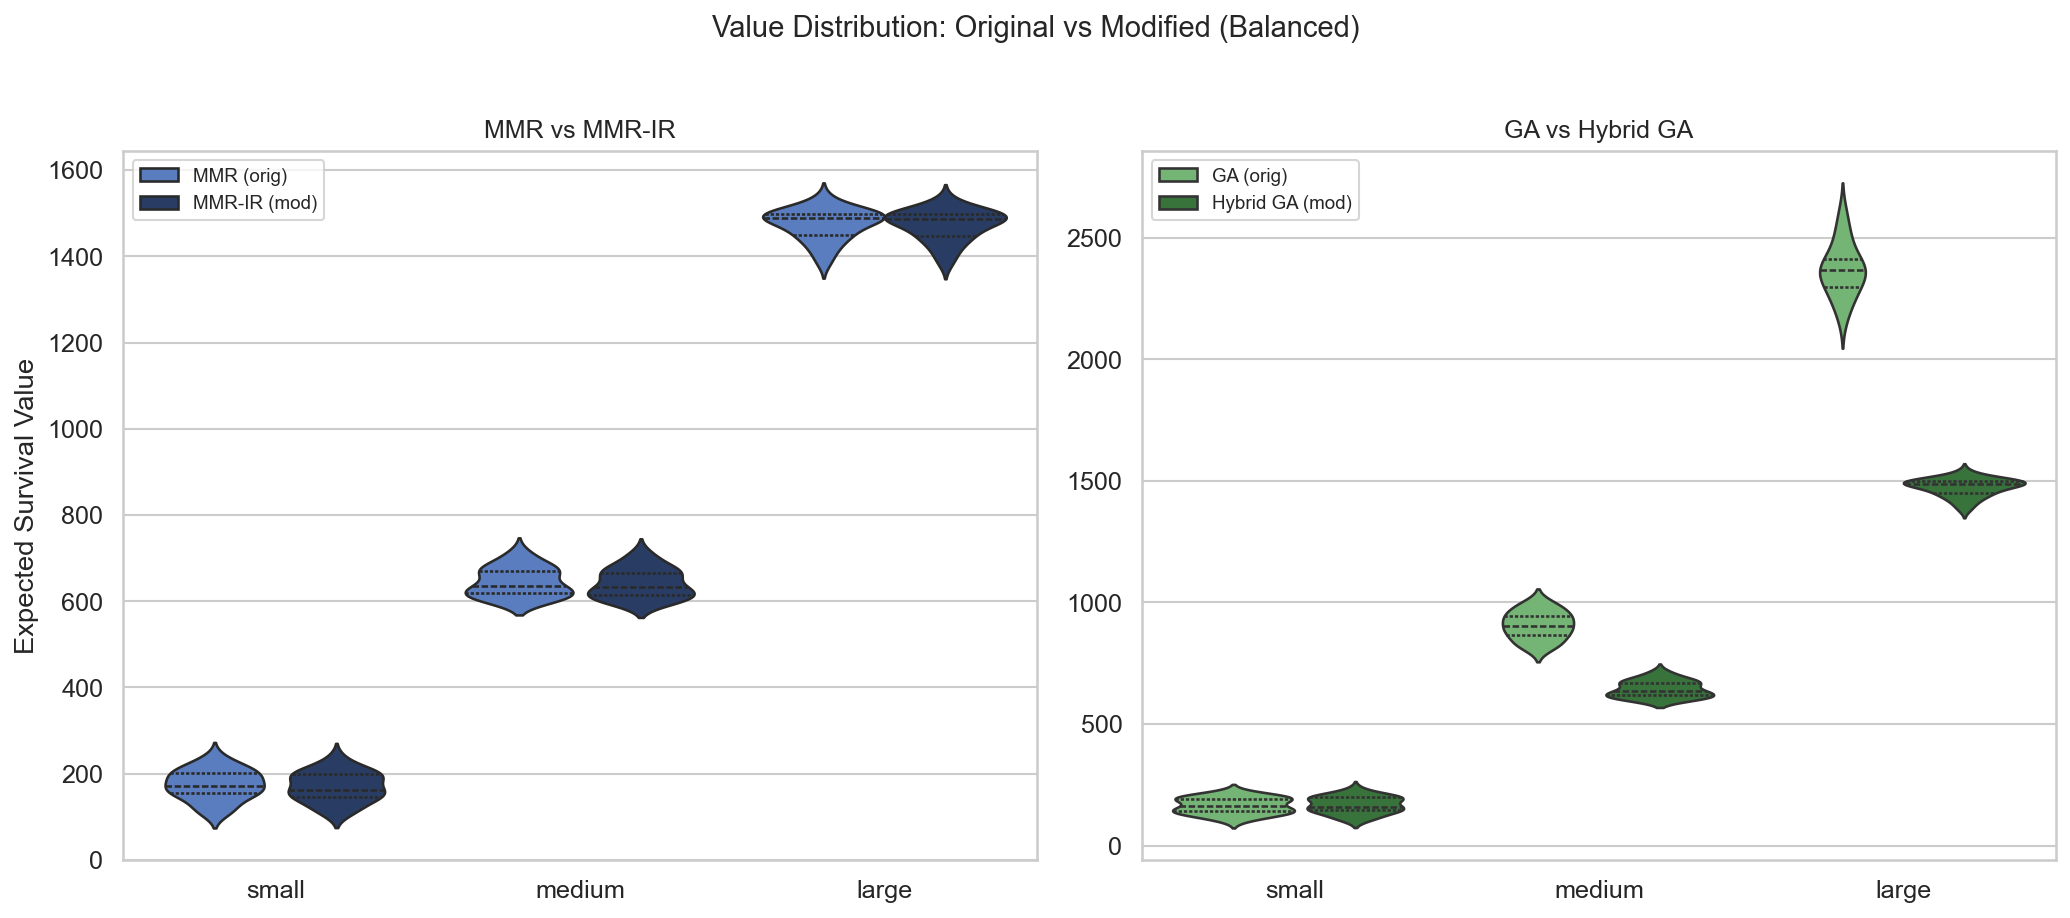
\includegraphics[width=0.92\textwidth]{images/07_violin_value_dist.png}
\end{center}

\vspace{-0.2cm}
{\footnotesize Violin plots showing the distribution of objective values for original vs. modified algorithms.}
\end{frame}

\begin{frame}{Results: Improvement by Scenario}
\begin{center}
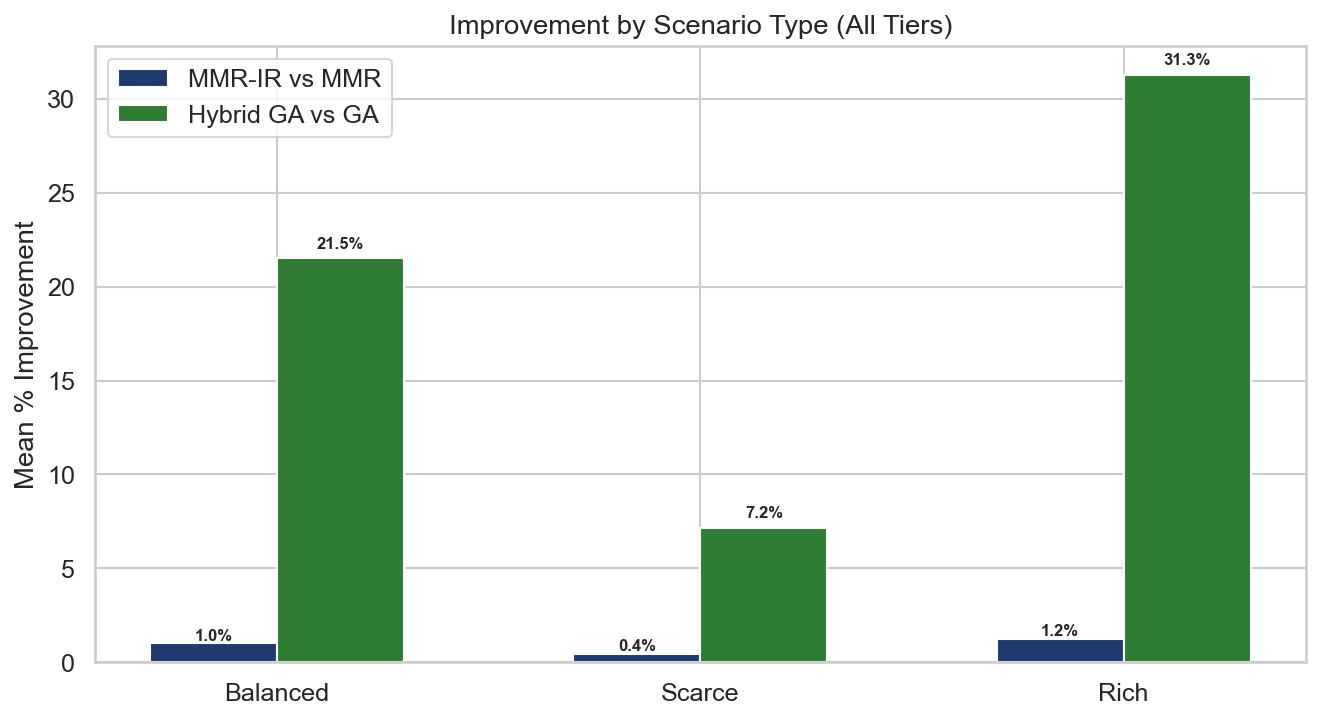
\includegraphics[width=0.92\textwidth]{images/08_bar_scenario_improvement.png}
\end{center}

\vspace{-0.2cm}
{\footnotesize Improvement percentage broken down by scenario type (balanced, scarce, rich).}
\end{frame}

\begin{frame}{Results: GA Improvement vs. Problem Size}
\begin{center}
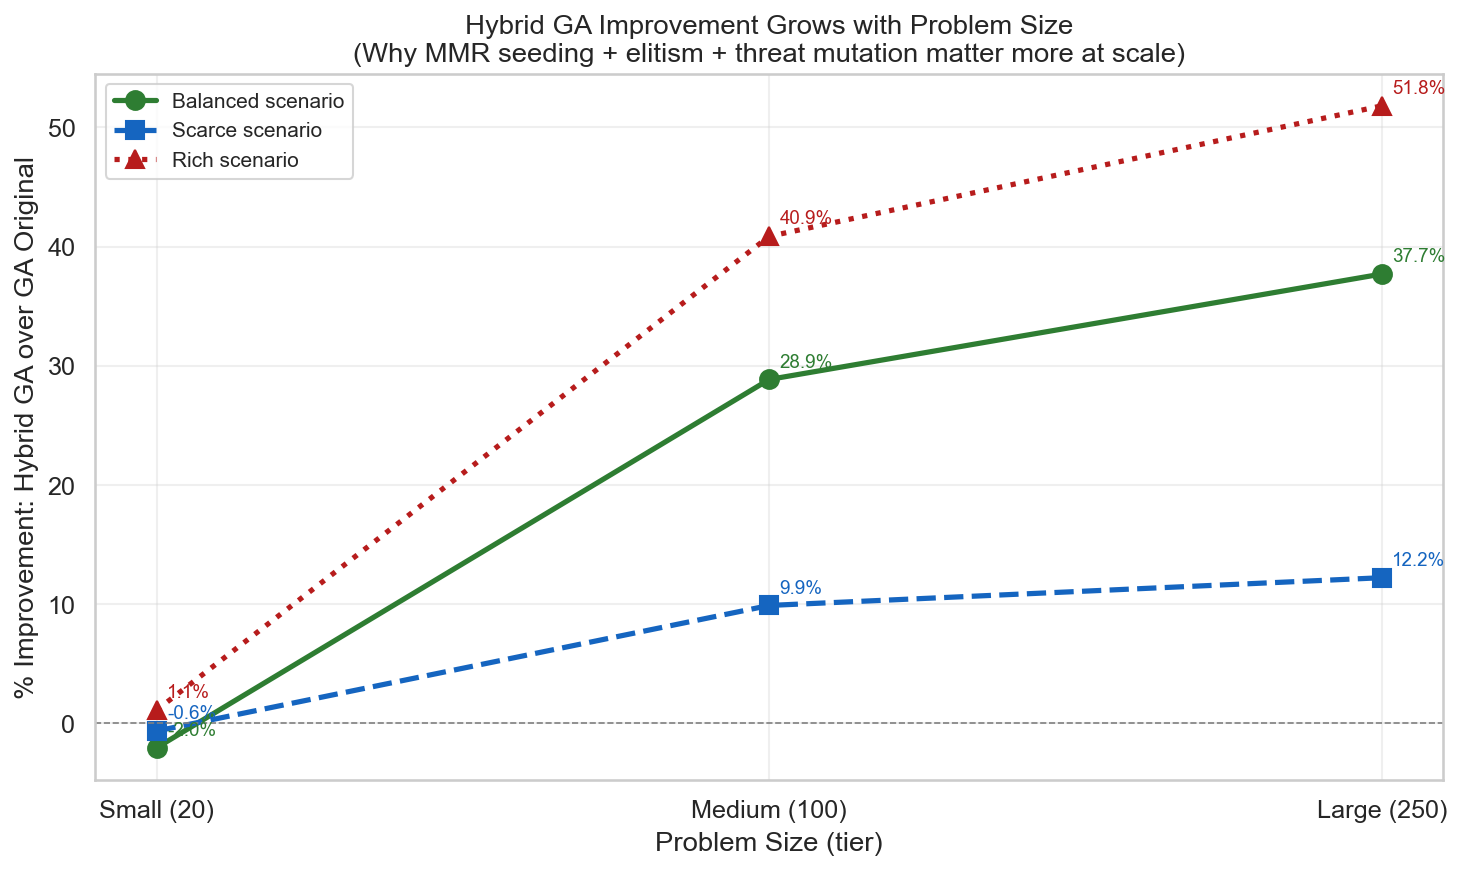
\includegraphics[width=0.92\textwidth]{images/09_ga_improvement_vs_size.png}
\end{center}

\vspace{-0.2cm}
{\footnotesize \textbf{Key finding:} Hybrid GA improvement over standard GA grows dramatically with problem size -- from $\sim$-2\% (small) to $\sim$52\% (large).}
\end{frame}

\begin{frame}{Key Findings}
\begin{block}{MMR-IR vs MMR (Original)}
\begin{itemize}
    \item \textbf{Consistent improvement:} 0.1--3.1\% across all tiers and scenarios
    \item 1-opt and 2-opt local search reliably escape greedy suboptimality
    \item Negligible additional runtime (local search is $O(1)$ per trial)
\end{itemize}
\end{block}

\begin{alertblock}{Hybrid GA vs GA (Original) -- The Main Story}
\begin{itemize}
    \item \textbf{Small:} -2--1\% improvement (modest)
    \item \textbf{Medium:} 10--41\% improvement (significant)
    \item \textbf{Large:} \textbf{12--52\% improvement} (dramatic)
    \item Improvement \textbf{grows with problem size} -- exactly where it matters most
\end{itemize}
\end{alertblock}

\begin{exampleblock}{Statistical Significance}
Wilcoxon signed-rank test ($\alpha = 0.05$): All pairwise comparisons between original and modified algorithms are \textbf{statistically significant} across all tiers.
\end{exampleblock}
\end{frame}

\begin{frame}{Why GA (Original) Fails at Scale}
\begin{alertblock}{Root Cause Analysis}
Three compounding factors explain why standard GA underperforms on medium/large instances:
\end{alertblock}

\vspace{0.2cm}
\begin{enumerate}
    \item \textbf{Large population, limited time:}
    \begin{itemize}
        \item Population size $= \max(W, T)$. For large\_rich: $\max(375, 250) = 375$ individuals
        \item With 60s time budget: only $\sim$160 generations completed
        \item 160 generations are insufficient to evolve 375-dimensional random solutions
    \end{itemize}

    \item \textbf{Random initialization:}
    \begin{itemize}
        \item All individuals start as random assignments -- far from any good solution
        \item In 375-dimensional space, random solutions have extremely high objective values
    \end{itemize}

    \item \textbf{No elitism:}
    \begin{itemize}
        \item The best solution found in early generations can be \textbf{lost}
        \item Replaced by offspring that may be worse
    \end{itemize}
\end{enumerate}

\vspace{0.2cm}
\begin{block}{Our Hybrid GA Fixes All Three}
MMR seed (warm start) + Elitism (preservation) + Threat-proportional mutation (guided search)
\end{block}
\end{frame}

\begin{frame}{Results Summary Table}
\begin{table}[h]
\centering
\small
\begin{tabular}{lrrrr}
\toprule
\textbf{Category} & \textbf{MMR (orig)} & \textbf{MMR-IR} & \textbf{GA (orig)} & \textbf{Hybrid GA} \\
\midrule
small\_balanced & 174 & 170 & 165 & 168 \\
small\_scarce & 475 & 471 & 462 & 465 \\
small\_rich & 74.5 & 72.2 & 72.1 & 71.2 \\
\midrule
medium\_balanced & 645 & 642 & 907 & 645 \\
medium\_scarce & 2085 & 2079 & 2310 & 2082 \\
medium\_rich & 243 & 243 & 412 & 243 \\
\midrule
large\_balanced & 1475 & 1473 & 2369 & 1474 \\
large\_scarce & 5169 & 5164 & 5888 & 5169 \\
large\_rich & 549 & 549 & 1140 & 549 \\
\bottomrule
\end{tabular}
\end{table}

\vspace{0.2cm}
{\footnotesize Mean objective values (lower = better). \textbf{Bold observation:} GA (orig) diverges dramatically on medium/large tiers. Hybrid GA brings it back to MMR-level performance. MMR-IR consistently improves over MMR by small but statistically significant margins.}
\end{frame}

% =============================================================================
% SECTION 7: REPRODUCIBILITY
% =============================================================================
\section{Reproducibility}

\begin{frame}[fragile]{Reproducibility: GitHub Repository}
\begin{block}{Single Master Script}
All experiments are reproducible with a single command:
\begin{center}
\texttt{python run\_all.py}
\end{center}
Generates dataset $\rightarrow$ runs all 4 algorithms on 180 instances $\rightarrow$ produces 9 plots.

\textbf{Runtime:} $\sim$3.5 hours total.
\end{block}

\vspace{0.2cm}
\begin{exampleblock}{Repository Structure}
\small
\begin{verbatim}
CSE_462-Algorithm-Engineering-Sessional/
  codes/
    run_all.py           # Master script
    dataset_generator.py # 180 instances
    experiment_runner.py # Run all algorithms
    analysis.py          # 9 plots + stats
    mmr_original.py      # MMR (Hasan & Barua)
    mmr_modified.py      # MMR-IR (ours)
    ga_original.py       # GA (Hasan & Barua)
    ga_modified.py       # Hybrid GA (ours)
  datasets/              # JSON instances
  results/figures/       # 9 PNG plots
\end{verbatim}
\end{exampleblock}
\end{frame}

\begin{frame}{GitHub Link}
\begin{center}
\vspace{1cm}
{\Large\textbf{GitHub Repository:}}

\vspace{0.5cm}
{\large\url{https://github.com/Arimotokika/CSE_462-Algorithm-Engineering-Sessional}}

\vspace{1cm}
\begin{block}{Quick Test (5 instances, $\sim$1 minute)}
\begin{center}
\texttt{python experiment\_runner.py --categories small\_balanced --instances 1-5}

\texttt{python analysis.py}
\end{center}
\end{block}
\end{center}
\end{frame}

% =============================================================================
% REFERENCES
% =============================================================================
\section{References}

\begin{frame}{References}
\begin{columns}[t]
\column{0.48\textwidth}
\scriptsize
\begin{thebibliography}{99}
\bibitem{intechopen2020}
Hasan, M. \& Barua, A. (2020). \textit{Weapon Target Assignment}. IntechOpen. DOI: 10.5772/intechopen.93665

\bibitem{ahuja2007}
Ahuja, R. K., et al. (2007). \textit{Exact and heuristic algorithms for the weapon-target assignment problem}. Operations Research.

\bibitem{lee2003}
Lee, Z. J., et al. (2003). \textit{Efficiently solving general weapon-target assignment problem by genetic algorithms with greedy eugenics}. IEEE Trans. SMC.

\bibitem{manne1958}
Manne, A. S. (1958). \textit{A target-assignment problem}. Operations Research.

\bibitem{bertsimas2025}
Bertsimas, D., et al. (2025). \textit{Solving large-scale WTA using branch-price-and-cut}. Naval Research Logistics.
\end{thebibliography}

\column{0.48\textwidth}
\scriptsize
\begin{thebibliography}{99}
\setcounter{enumiv}{5}
\bibitem{andersen2022}
Andersen, A. C., et al. (2022). \textit{The weapon-target assignment problem: Exact and approximate algorithms}. Ann. Oper. Res.

\bibitem{kwon1999}
Kwon, O., et al. (1999). \textit{A Lagrangian relaxation approach to targeting}. Naval Research Logistics.

\bibitem{kline2020}
Kline, A. G., et al. (2020). \textit{Heuristic and metaheuristic for static weapon-target assignment}. J. Global Optim.

\bibitem{lee2002}
Lee, Z. J., et al. (2002). \textit{Immunity-based ant colony optimization for weapon-target assignment}. Applied Soft Computing.

\bibitem{lloyd1986}
Lloyd, S. P., et al. (1986). \textit{Weapons allocation is NP-complete}. IEEE.
\end{thebibliography}
\end{columns}
\end{frame}

% =============================================================================
% THANK YOU
% =============================================================================

\begin{frame}[plain]
\begin{center}
\vspace{2cm}
{\Huge\textbf{\textcolor{primaryblue}{Thank You!}}}

\vspace{1cm}
{\Large Questions?}

\end{center}
\end{frame}

\end{document}
